\documentclass[ALICE,manyauthors]{cernphprep}

%%%%%%%% Shorthand definitions %%%%%%%%%%%%%%%%%%%%%%%%%%%%%%%%%%%%%%%%%%%%%%%%%%%%%%%%%%%%%
\newcommand{\kstar}{$k^{*}$\xspace}
\newcommand{\ktrue}{$k^{*}_{\mathrm{True}}$\xspace}
\newcommand{\krec}{$k^{*}_{\mathrm{Rec}}$\xspace}
\newcommand{\minv}{$m_{\mathrm{inv}}$\xspace}
\newcommand{\mt}{$m_{\mathrm{T}}$\xspace}
\newcommand{\pt}{$p_{\mathrm{T}}$\xspace}

\newcommand{\Lam}{$\Lambda$\xspace}
\newcommand{\ALam}{$\bar{\Lambda}$\xspace}
\newcommand{\LamALam}{$\Lambda$($\bar{\Lambda}$)\xspace}

\newcommand{\KchP}{$\mathrm{K^{+}}$\xspace}
\newcommand{\KchM}{$\mathrm{K^{-}}$\xspace}
\newcommand{\Kpm}{$\mathrm{K^{\pm}}$\xspace}

\newcommand{\Ks}{$\mathrm{K^{0}_{S}}$\xspace}

\newcommand{\LamK}{$\Lambda$K\xspace}
\newcommand{\ALamAK}{$\bar{\Lambda}\bar{\mathrm{K}}$\xspace}


\newcommand{\LamKchP}{$\Lambda\mathrm{K^{+}}$\xspace}
\newcommand{\ALamKchM}{$\bar{\Lambda}\mathrm{K^{-}}$\xspace}
\newcommand{\LamKchPALamKchM}{$\Lambda\mathrm{K^{+}}$($\bar{\Lambda}\mathrm{K^{-}}$)\xspace}

\newcommand{\LamKchM}{$\Lambda\mathrm{K^{-}}$\xspace}
\newcommand{\ALamKchP}{$\bar{\Lambda}\mathrm{K^{+}}$\xspace}
\newcommand{\LamKchMALamKchP}{$\Lambda\mathrm{K^{-}}$($\bar{\Lambda}\mathrm{K^{+}}$)\xspace}

\newcommand{\LamKpm}{$\Lambda\mathrm{K^{\pm}}$\xspace}
\newcommand{\ALamKpm}{$\bar{\Lambda}\mathrm{K^{\pm}}$\xspace}
\newcommand{\LamALamKpm}{$\Lambda$($\bar{\Lambda}$)$\mathrm{K^{\pm}}$\xspace}


\newcommand{\LamKs}{$\Lambda\mathrm{K^{0}_{S}}$\xspace}
\newcommand{\ALamKs}{$\bar{\Lambda}\mathrm{K^{0}_{S}}$\xspace}
\newcommand{\LamKsALamKs}{$\Lambda\mathrm{K^{0}_{S}}$($\bar{\Lambda}\mathrm{K^{0}_{S}}$)\xspace}
\newcommand{\LamALamKs}{$\Lambda$($\bar{\Lambda}$)$\mathrm{K^{0}_{S}}$\xspace}

\newcommand{\XiKchP}{$\Xi^{-}\mathrm{K^{+}}$\xspace}
\newcommand{\AXiKchM}{$\bar{\Xi}^{+}\mathrm{K^{-}}$\xspace}

\newcommand{\XiKchM}{$\Xi^{-}\mathrm{K^{-}}$\xspace}
\newcommand{\AXiKchP}{$\bar{\Xi}^{+}\mathrm{K^{+}}$\xspace}


\newcommand{\XiKpm}{$\Xi^{-}\mathrm{K^{\pm}}$\xspace}
\newcommand{\AXiKpm}{$\bar{\Xi}^{+}\mathrm{K^{\pm}}$\xspace}
%%%%%%%%%%%%%%%%%%%%%%%%%%%%%%%%%%%%%%%%%%%%%%%%%%%%%%%%%%%%%%%%%%%%%%%%%%%%%%%%%%%%%%%%%%%%

\usepackage[comma,square,numbers,sort&compress]{natbib}
\usepackage{hyperref}
\usepackage{lineno}
%\linenumbers

\usepackage{multirow}
\usepackage{boldline}  % to make lines in table bold

\usepackage{pdflscape}

\usepackage{comment}

\begin{document}%

%%%%%%%%%%%%%%%  Title page %%%%%%%%%%%%%%%%%%%%%%%%
\begin{titlepage}
%
\PHyear{2015}
\PHnumber{XXX}      % required, will be obtained from PH
\PHdate{Day Month}  % required, will be obtained from PH
%

%%% Put your own title + short title here:
\title{\LamK femtoscopy in Pb-Pb collisions at $\sqrt{s_{\mathrm{NN}}} = $ 2.76 TeV}
\ShortTitle{\LamK femtoscopy in Pb-Pb collisions}   % appears on right page headers

%%% Do not change the next lines
\Collaboration{ALICE Collaboration\thanks{See Appendix~\ref{app:collab} for the list of collaboration members}}
\ShortAuthor{ALICE Collaboration} % appears on left page headers, do not change

\begin{abstract}
We present our femtoscopy analysis of \LamK correlations in Pb-Pb collisions at $\sqrt{s_{\mathrm{NN}}}$ = 2.76 TeV from ALICE.  
The femtoscopic correlations result from strong final-state interactions, and are fit with a parametrization based on a model by Lednicky and Lyuboshitz.  
This allows us to both characterize the emission source and measure the scattering parameters for the particle pairs.  
We observe a large difference in the \LamKchP and \LamKchM correlations in pairs with low relative momenta.  
This might suggest an effect arising from different quark-antiquark interactions between the pairs ($\mathrm{s}\bar{\mathrm{s}}$ in \LamKchP and $\mathrm{u}\bar{\mathrm{u}}$ in \LamKchM), or from different net strangeness for each system.
\end{abstract}
\end{titlepage}
\setcounter{page}{2}

\section{Introduction}
\label{sec:Introduction}

Femtoscopy is an experimental method used to study the space-time characteristic of the particle emitting sources in relativistic particle collisions \cite{Lisa:2005dd}.  With this method, two(or many)-particle relative-momentum correlation functions are used to connect the final-state momentum distributions to the space-time distributions of particle emission at freeze-out.  The correlation functions are sensitive to quantum statistics, as well as strong and Coulomb final-state interactions (FSI).  In addition to characterizing the source region, femtoscopy offers a unique opportunity to measure nuclear scattering parameters, many of which are difficult, if not impossible, to measure otherwise.  In many pair systems, the contributions to the correlation function from quantum statistics and/or the Coulomb interaction overwhelm that of the strong interaction, making it difficult to extract scattering information.  In this article, we study npn-identical particle pairs, with at least one electrically neutral particle in the pair.  Therefore, quantum statistics and the Coulomb interaction do not contribute, giving us a clear signal from the strong interaction.

Femtoscopy analyses of pion, kaons, and protons have revealed a trend of decreasing source radii with increasing transverse mass, $m_{\mathrm{T}}^{2} = (\frac{m_{\mathrm{inv}}}{2})^{2} + k_{\mathrm{T}}^{2}$, where $k_{\mathrm{T}} = \frac{1}{2}|\mathbf{p}_{\mathrm{T},1} + \mathbf{p}_{\mathrm{T},2}|$.  This is interpreted as a signature of hydrodynamic flow, and therefore deconfined quark matter, in the heavy-ion collisions.

We observe mT-scaling.  However, remember plot is for identical particle femtoscopy.  When dealing with \LamK, don't necessarily expect exact same trend.  mT-scaling has to do with hydro, and single particle distributions.  With femtoscopy, we are dealing with pairs of particles.  If we look at \LamK as a function of mT, we certainly would expect a decreasing behavior with increasing mT, but the exact shape may not be same of pipi, kk, pp, etc.


Motivation for comparing studies with different particle species, and for \LamK in particular.

Note, we expect and observe consistent results between a particle pair and its conjugate (ex. \LamKchP and \ALamKchM); therefore, we group the two together as a single analysis, and will refer to the joined analysis by the pair name, excluding the conjugate.  
So, for instance, \LamKs $\oplus$ \ALamKs is simply \LamKs, \LamKchP $\oplus$ \ALamKchM is \LamKchP, etc. 


This paper presents results from a femtoscopic analysis of \LamK correlations in Pb-Pb collisions at $\sqrt{s_{\mathrm{NN}}}$ = 2.76 TeV by the ALICE experiment at the LHC.  
All pair combinations of \Lam and \ALam with \KchP, \KchM and \Ks are analyzed. 
The femtoscopic correlations are the result of strong final-state interactions, and are fit with a parametrization based on a model by R. Lednicky and V. L. Lyuboshitz \cite{Lednicky:82}.  
This allows us to both characterize the emission source and measure the scattering parameters for the particle pairs.  
We observe a large difference in the \LamKchPALamKchM and \LamKchMALamKchP correlations in pairs with low relative momenta (\kstar $\lesssim$ 100 MeV).  
The results suggest an effect arising from different quark-antiquark interactions in the pairs, i.e. $\rm s\bar{s}$ in \LamKchPALamKchM and $\rm u\bar{u}$ in \LamKchMALamKchP.  
The femtoscopic radii, $\lambda$ parameters, and scattering parameters are extracted from...

The organization of this paper is as follows.  Sec. \ref{sec:DataAnalysis}, Sec. \ref{sec:AnalysisMethods}, Sec. \ref{sec:Results}, Sec. \ref{sec:Summary}.

\section{Data Analysis}
\label{sec:DataAnalysis}

The dataset analyzed is from Pb-Pb collisions at $\sqrt{s_{\mathrm{NN}}}$ = 2.76 TeV at the LHC measured by the ALICE detector \cite{1748-0221-3-08-S08002}.
Approximately 40 million combined central, semi-central, and minimum bias events were analyzed.
The events were classified according to their centrality determined using the measured amplitudes in the V0 detectors \cite{Abelev:2013qoq}.  
In order for an event to be included in the analysis, the z-position of the reconstructed event vertex must be within 10 cm of the center of the ALICE detector, and the event must contain at least one particle of each type from the pair of interest (ex. for \LamKchP analysis, an accepted event must contain at least one \Lam and at lease one \Ks). 

Charged particle tracking was performed using the Time Projection Chamber (TPC) \cite{2010NIMPA.622..316A} (Tom) or \cite{Dellacasa:451098} (1dPionKaonProton) and the Inner Tracking System \cite{1748-0221-3-08-S08002}.  
The ITS allows for high spatial resolution in determining the primary (collision) vertex.
The determination of the momenta of the tracks was performed using tracks reconstructed with the TPC only and constrained to the primary vertex.
A minimum requirement on the number of reconstructed TPC clusters was imposed, the purpose of which is to ensure both the quality of the track and good \pt resolution at large momenta, as well as to remove fake tracks.

Particle identification (PID) for reconstructed tracks was carried out using both the TPC and Time-of-Flight (TOF) detector \cite{Abelev:2014ffa, Akindinov:2013tea} (Tom) or \cite{Cortese:545834} (1dPionKaonProton) in the pseudorapidity range $|\eta| < 0.8$.  
For TPC PID, a parametrized Bethe-Bloch formula was used to calculate the specific energy loss $\langle \mathrm{d}E/\mathrm{d}x \rangle$ in the detector expected for a particle with a given mass and momentum.  
For TOF PID, the particle mass was used to calculate the expected time-of-flight as a function of track length and momentum.  
For each PID method, a value ($N\sigma$) was assigned to each track denoting the number of standard deviations between the measured track information and calculated values.  
This procedure was repeated for four "particle species hypotheses" - electron, pion, kaon, and proton-, and, for each hypothesis, a different $N\sigma$ value was obtained per detector.


\subsection{K$^{\pm}$ selection}
\label{sec:KchSelection}
The single-particle selection criteria used to select charged kaon candidates are summarized in Table \ref{tab:KchCuts}.
\Kpm track detection utilized both TPC and TOF detectors, and tracks within the range 0.14 $<$ \pt $<$ 1.5 GeV/$c$ were accepted.
As we are interested in primary particles originating from the primary vertex, to reduce the number of secondaries (for instance, charged particles produced in the detector material, particles from weak decays, etc.) in our sample, we established a maximum cut on the distance-of-closest-approach (DCA) of the track the the primary vertex.
This restriction is realized by imposing a DCA cut in both the transverse and beam directions.

PID was performed using both the TPC and TOF detectors via the $\mathrm{N}\sigma$ method.  
The exact cuts for the various \pt regions can be found in Table \ref{tab:KchCuts}.  
Additionally, we include methods to reduce the contamination in our \Kpm samples from electrons and pions.  Again, the specifics for these cuts are contained in Table \ref{tab:KchCuts}.


\begin{figure}[h]
 \centering
 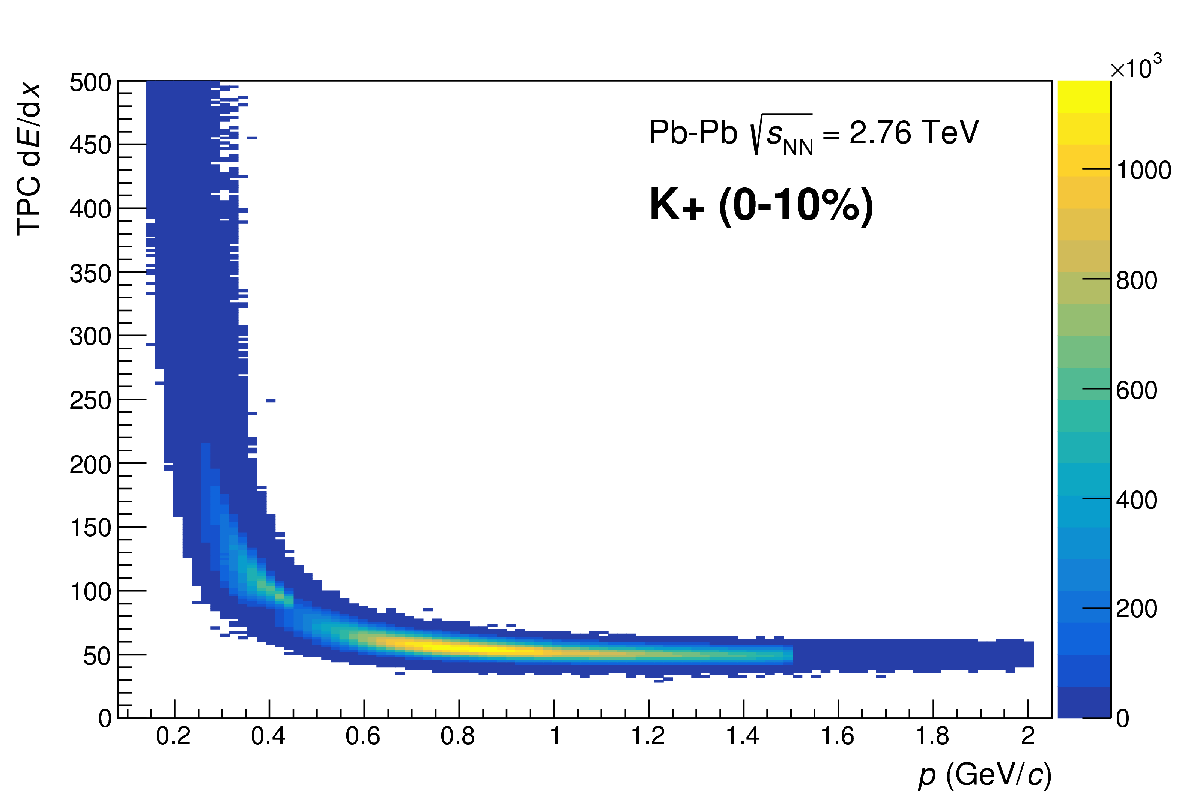
\includegraphics[width=0.5\textwidth]{/home/jesse/Analysis/FemtoAnalysis/LamKPublication/Figures/PDF/canDrawKchdEdx_LamKchP_0010_KchP.pdf}% Here is how to import EPS art
 \caption{\label{fig:KchPdEdx} Sample d$E$/d$x$ distribution for the \KchP collection from our 0-10\% central \LamKchP analysis.}
\end{figure}

\begin{table}[htbp]
 \centering
%  \renewcommand{\arraystretch}{1.5}
  \begin{tabular}{lc|c|l}
   \hline  
   \multicolumn{4}{c}{\textbf{\Kpm selection}} \\
   \hline
   \multicolumn{3}{l|}{Transverse momentum $p_{\mathrm{T}}$} & 0.14 $< p_{\mathrm{T}} < 1.5$ GeV/\textit{c} \\
   \hline
   \multicolumn{3}{l|}{$|\eta|$} & $< 0.8$ \\
   \hline
   \multicolumn{3}{l|}{Transverse DCA to primary vertex} & $<$ 2.4 cm \\
   \hline
   \multicolumn{3}{l|}{Longitudinal DCA to primary vertex} & $<$ 3.0 cm \\
   \hline

   TPC and TOF N$\sigma$ Cuts & \multicolumn{3}{c}{} \\
   \cline{2-4}
    & \multicolumn{1}{l}{$p <$ 0.4 GeV/\textit{c}} &  & N$_{\sigma \mathrm{K,TPC}} <$ 2 \\
   \cline{2-4}
    & \multicolumn{1}{l}{0.4 $< p <$ 0.45 GeV/\textit{c}} & & N$_{\sigma \mathrm{K,TPC}} <$ 1 \\
   \cline{2-4}     
    & \multicolumn{1}{l}{0.45 $< p <$ 0.80 GeV/\textit{c}} & & N$_{\sigma \mathrm{K,TPC}} <$ 3 \\ 
   \multicolumn{3}{c|}{} & N$_{\sigma \mathrm{K,TOF}} <$ 2 \\
   \cline{2-4}
    & \multicolumn{1}{l}{0.80 $< p <$ 1.0 GeV/\textit{c}} & & N$_{\sigma \mathrm{K,TPC}} <$ 3 \\
   \multicolumn{3}{c|}{} & N$_{\sigma \mathrm{K,TOF}} <$ 1.5 \\  
   \cline{2-4}
    & \multicolumn{1}{l}{$p >$ 1.0 GeV/\textit{c}} & & N$_{\sigma \mathrm{K,TPC}} <$ 3 \\
   \multicolumn{3}{c|}{} & N$_{\sigma \mathrm{K,TOF}} <$ 1 \\  
   \hline
   \multicolumn{3}{l|}{\multirow{3}{*}{Electron Rejection: Reject if all satisfied}} & $\mathrm{N}_{\sigma e^{-},\mathrm{TPC}} < $ 3 \\
   \multicolumn{3}{c|}{} & $\mathrm{N}_{\sigma e^{-},\mathrm{TPC}} < \mathrm{N}_{\sigma K^{\pm},\mathrm{TPC}}$ \\
   \multicolumn{3}{c|}{} & $\mathrm{N}_{\sigma e^{-},\mathrm{TOF}} < \mathrm{N}_{\sigma K^{\pm},\mathrm{TOF}}$ \\
   \hline
   
   \multicolumn{4}{l}{Pion Rejection:  Reject if:} \\
   %\cline{1-1}
   \multirow{4}{*}{$p <$ 0.65 GeV/\textit{c}} & \multicolumn{1}{l}{TOF and TPC available} & \multicolumn{1}{c|}{} & N$_{\sigma \pi,\mathrm{TPC}} <$ 3 \\
   \multicolumn{3}{c|}{} & N$_{\sigma \pi,\mathrm{TOF}} <$ 3 \\
   \cline{2-4}
    & \multirow{2}{*}{Only TPC available} & $p <$ 0.5 GeV/\textit{c} & N$_{\sigma \pi,\mathrm{TPC}} <$ 3 \\
   \cline{3-4}
    &  & 0.5 $< p <$ 0.65 GeV/\textit{c} & N$_{\sigma \pi,\mathrm{TPC}} <$ 2 \\
   \cline{2-4}
   \multicolumn{3}{l|}{\multirow{2}{*}{0.65 $< p <$ 1.5 GeV/\textit{c}}} & N$_{\sigma \pi,\mathrm{TPC}} <$ 5 \\
    & \multicolumn{2}{c|}{} & N$_{\sigma \pi,\mathrm{TOF}} <$ 3 \\
   \cline{2-4}
   \multicolumn{3}{l|}{\multirow{2}{*}{$p >$ 1.5 GeV/\textit{c}}} & N$_{\sigma \pi,\mathrm{TPC}} <$ 5 \\
    & \multicolumn{2}{c|}{} & N$_{\sigma \pi,\mathrm{TOF}} <$ 2 \\
   \hline
  \end{tabular}
% \end{minipage}
 \caption{\Kpm selection}
 \label{tab:KchCuts} 
\end{table}

The purity of the \Kpm collections was estimated from a Monte-Carlo (MC) study based on HIJING \cite{PhysRevD.44.3501} simulations using GEANT3 \cite{Brun:1994aa} to model particle transport through the ALICE detectors. In these simulations, the true identity of each reconstructed K$^{\pm}$ particle is known;  therefore, the purity may be estimated as:

\begin{equation}
 \rm Purity(K^{\pm}) = \frac{N_{true}}{N_{reconstructed}} \\
\label{eqn:KchPurity}
\end{equation}

For our analysis, we find Purity(\KchP) $\approx$ Purity(\KchM) $\approx$ 97\%.
Figure \ref{fig:KchPdEdx} shows a sample d$E$/d$x$ for the \KchP collection in the 0-10\% centrality bin (from our \LamKchP study).



\subsection{V0 selection}
\label{sec:V0Selection}

\LamALam and \Ks particles are electrically neutral, and cannot be directly detected, but must instead be reconstructed through detection of their decay products, or daughters.  
This process is illustrated in Figure \ref{fig:V0Reconstruction}, and the main cuts used are shown in Tables \ref{tab:LamCuts} and \ref{tab:K0sCuts}..
In general, particles which are topologically reconstructed in this fashion are called V0 particles.
The decay channel \Lam $\rightarrow$ p$\pi^{-}$ was used for the identification of \Lam hyperons (and, similarly the charge-conjugate decay for the \ALam identification), and \Ks $\rightarrow$ $\pi^{+}\pi^{-}$ for the identification of \Ks mesons.

\begin{figure}[h]
  \centering
  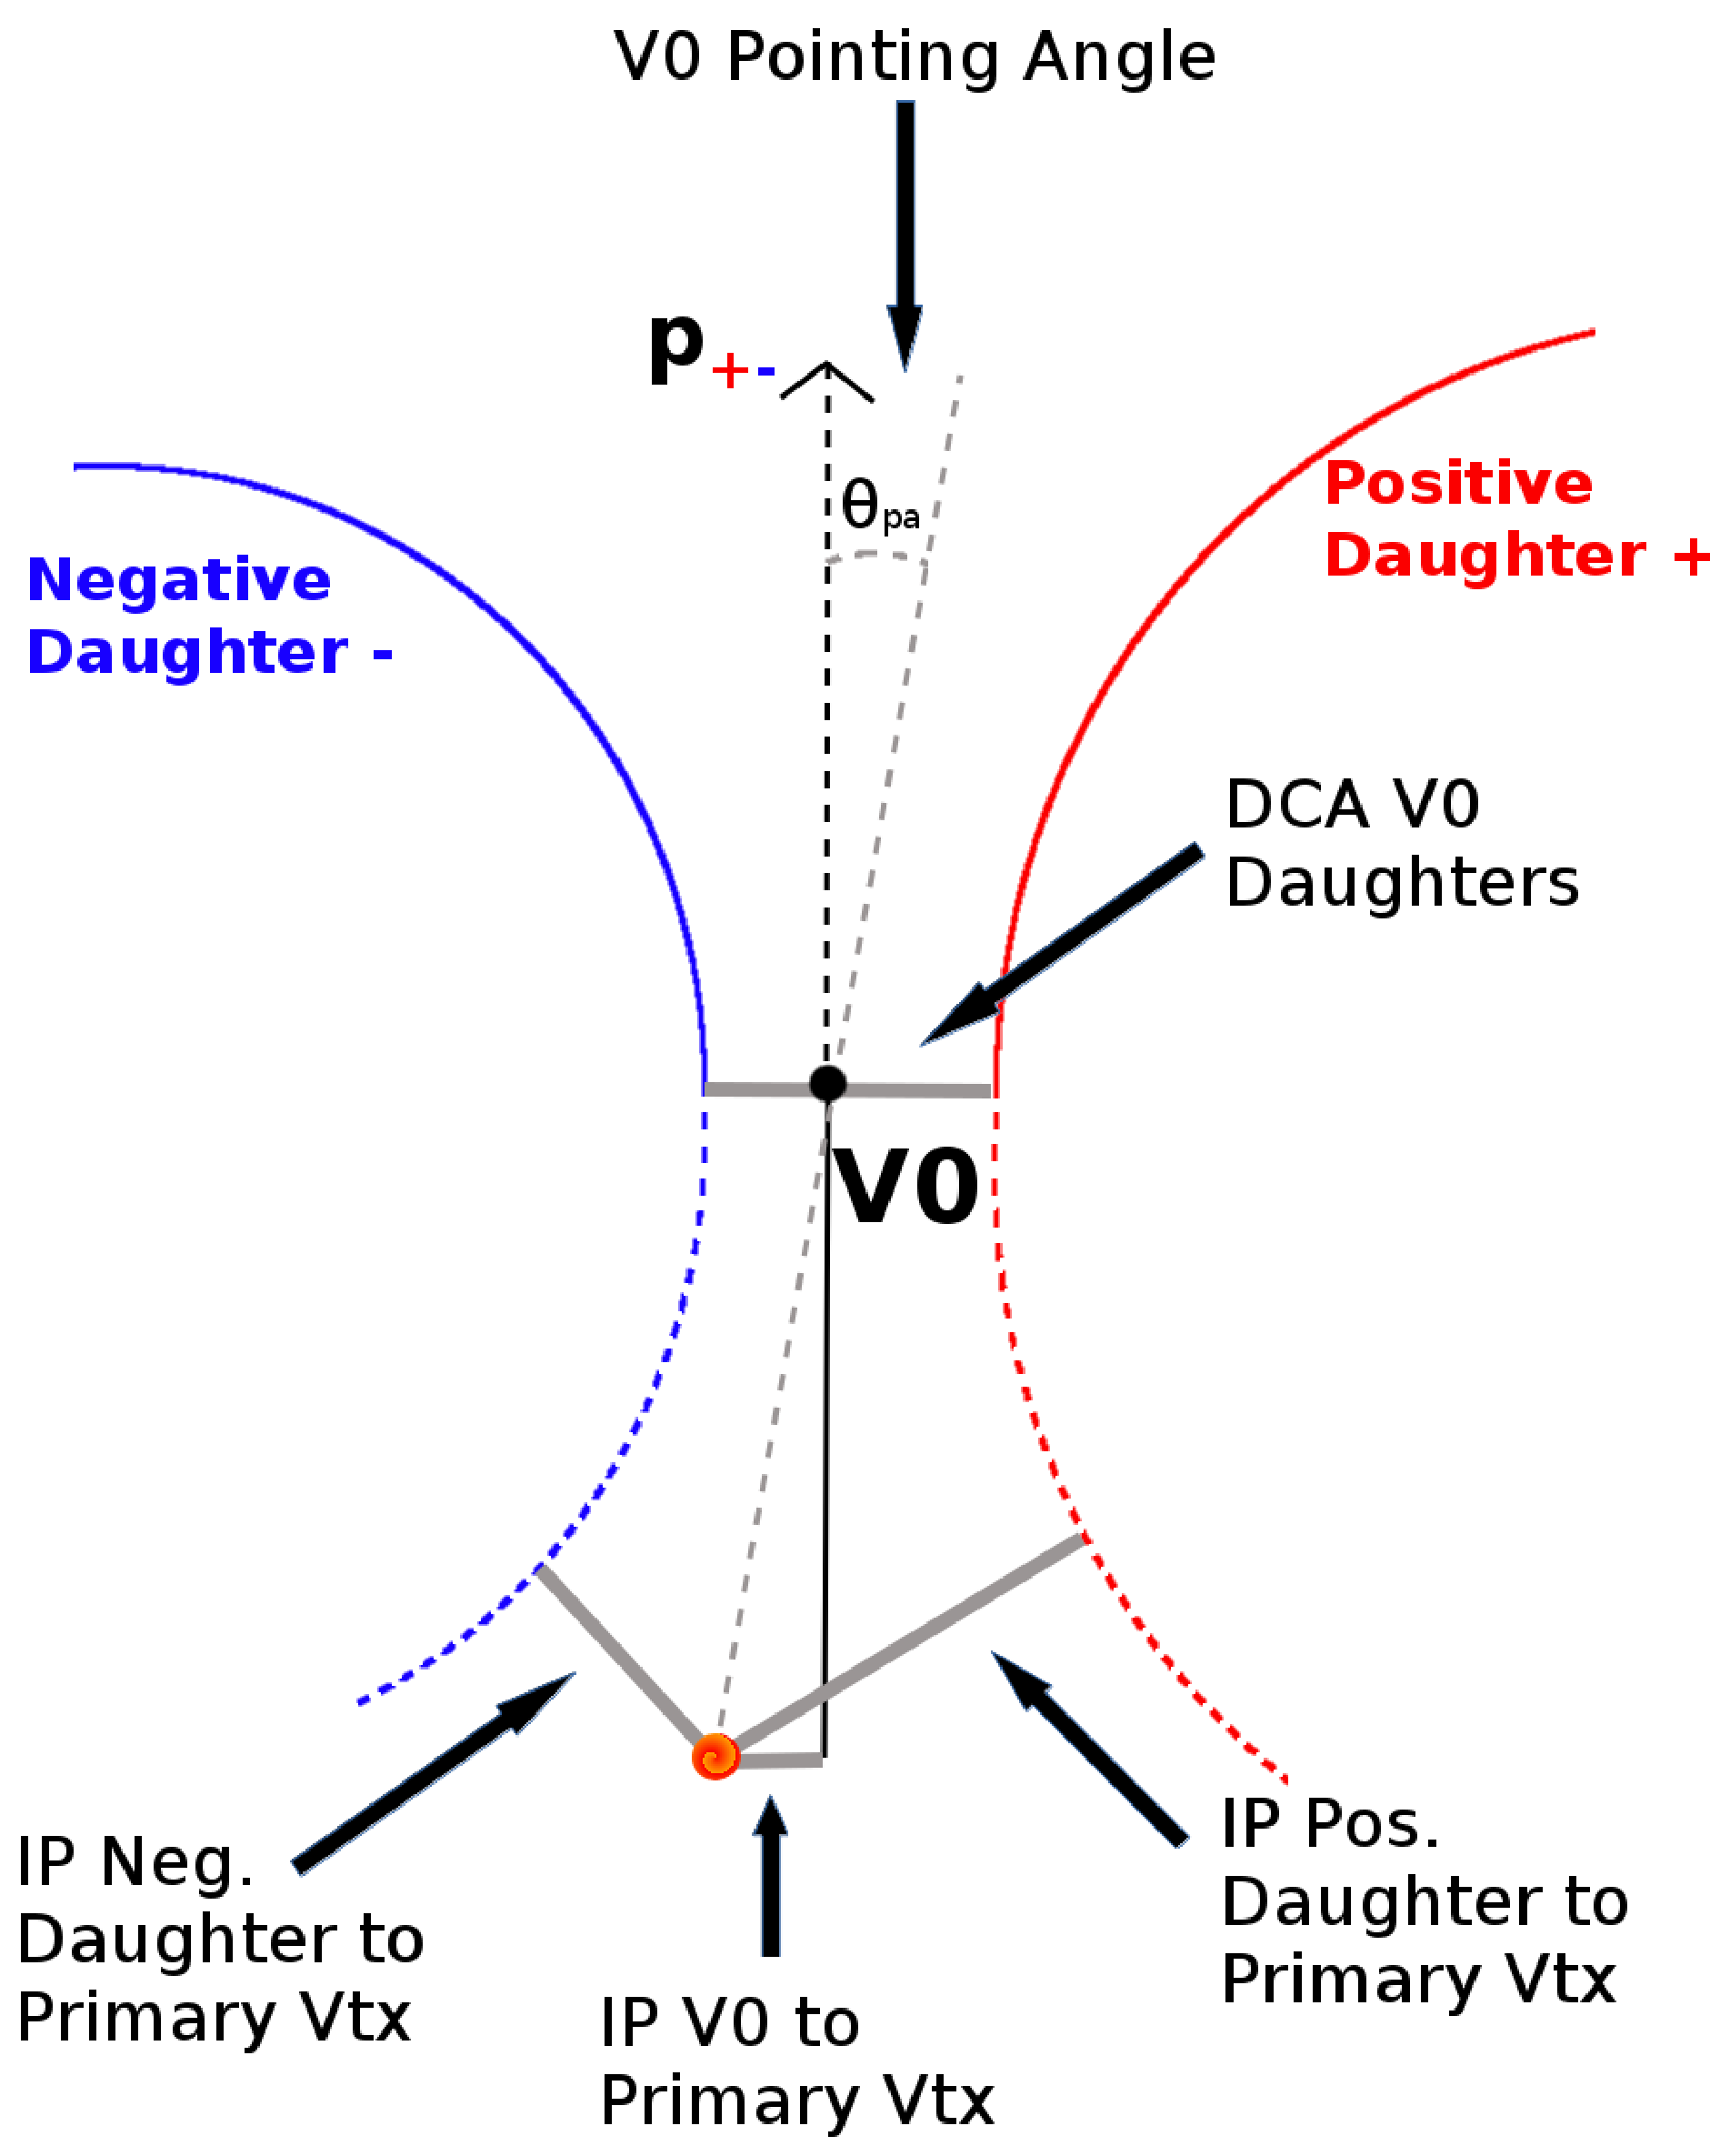
\includegraphics[width=0.30\textwidth]{/home/jesse/Analysis/FemtoAnalysis/LamKPublication/Figures/PDF/V0CutsGeneral.pdf}
  \caption[V0 Reconstruction]{V0 Reconstruction}
  \label{fig:V0Reconstruction}
\end{figure}

To construct a V0 particle, the charged daughter tracks must first be found.  
Aside from typical kinematic and PID cuts (using TPC and TOF detectors), the daughter tracks are also exposed to a minimum cut on the impact parameter with respect to the primary vertex.  
The daughters of a V0 particle should not originate from the primary vertex, but rather from the decay vertex of the V0, hence the minimum cut imposition.  The positive and negative daughter tracks are combined to form the V0 candidate, the momentum of which is simply the sum of the momenta of the daughters.
The decay vertex of the V0 is assumed to be the point of closest approach between the daughter tracks.
To help ensure quality, a maximum value cut is demanded on the distance-of-closest-approach between the daughters (DCA V0 Daughters).

A minimum transverse momentum cut on the V0 candidate is introduced to reduce contamination from fake candidates.
Opposite to the daughter tracks, the V0 candidate is exposed to a maximum cut on the impact parameter with respect to the primary vertex.
In this case, we do want our V0 candidates to be primary, hence the maximum cut imposition.
To further strengthen our selection of primary V0 candidates, we impose a selection on the pointing angle, $\theta_{\mathrm{pa}}$, between the V0 momentum and the vector pointing from the primary vertex to the secondary V0 decay vertex.
We want to V0 candidate's momentum to point back to the primary decay vertex, and therefor a small $\theta_{\mathrm{pa}}$; we achieve this by appointing a minimum value on $\cos(\theta_{\mathrm{pa}})$ (``Cosine of pointing angle'' in Tables \ref{tab:LamCuts} and \ref{tab:K0sCuts}).

On occasion, \LamALam particles are misidentified as \Ks, and vice versa.  
To attempt to remove these contaminations without throwing away good candidates, we impose a set of misidentification cuts.  
The intent of these cuts is to judge whether a candidate is more likely a \LamALam or a \Ks.  

For a given V0, we calculate the mass assuming different identities (\Lam, \ALam, \Ks); the mass assuming \Ks hypothesis ($m_{\mathrm{inv,~ K^{0}_{S}~ Hypothesis}}$) is calculated assuming both of the daughters are pions, the mass assuming \Lam hypothesis ($m_{\mathrm{inv,~ \Lambda~ Hypothesis}}$) is calculated assuming the positive daughter is a proton and the negative daughter a pion, and the mass assuming \ALam hypothesis ($m_{\mathrm{inv,~ \bar{\Lambda}~ Hypothesis}}$) is calculated assuming the positive daughter is a pion and the negative an anti-proton.  
In addition to the notation just introduced, in the following, $m_{\mathrm{PDG,~ K^{0}_{S}}}$ and $m_{\mathrm{PDG,~ \Lambda(\bar{\Lambda})}}$ denote the particle masses of the \Ks and \LamALam, respectively, as recorded by the Particle Data Group \cite{Patrignani:2016xqp}.

For \LamALam selection, a candidate is rejected if all of the following criteria are satisfied:

\begin{enumerate}
 \item $\left|m_{\mathrm{inv,~ K^{0}_{S}~ Hypothesis}} - m_{\mathrm{PDG,~ K^{0}_{S}}}\right| < $ 9.0 MeV/c$^{2}$
 \item Daughter particles pass daughter cuts intended for \Ks reconstruction
 \begin{enumerate}
  \item \Lam selection
  \begin{enumerate}
   \item p daughter passes $\pi^{+}$ cuts intended for \Ks reconstruction
   \item $\pi^{-}$ daughter passes $\pi^{-}$ cuts intended for \Ks reconstruction.
  \end{enumerate}
  \item \ALam selection
  \begin{enumerate}
   \item $\pi^{+}$ daughter passes $\pi^{+}$ cuts intended for \Ks reconstruction
   \item $\bar{\mathrm{p}}$ daughter passes $\pi^{-}$ cuts intended for \Ks reconstruction.
  \end{enumerate}  
 \end{enumerate}
 \item $\left|m_{\mathrm{inv,~ K^{0}_{S}~ Hypothesis}} - m_{\mathrm{PDG,~ K^{0}_{S}}}\right|~ < ~\left|m_{\mathrm{inv,~ \Lambda(\bar{\Lambda})~ Hypothesis}} - m_{\mathrm{PDG,~ \Lambda(\bar{\Lambda})}}\right|$
\end{enumerate} 

Similarly, for \Ks selection, a candidate is rejected if all of the following criteria are satisfied for the \Lam case, or for the \ALam case:

\begin{enumerate}
 \item $\left|m_{\mathrm{inv}, \ \Lambda(\bar{\Lambda}) \ \mathrm{Hypothesis}} - m_{\mathrm{PDG},\ \Lambda(\bar{\Lambda})}\right| < $ 9.0 MeV/$c^{2}$
 \item Daughter particles pass daughter cuts intended for \LamALam reconstruction
 \begin{enumerate}
  \item $\pi^{+}$ daughter passes p($\pi^{+}$) daughter cut intended for \LamALam reconstruction
  \item $\pi^{-}$ daughter passes $\pi^{-}$($\bar{\mathrm{p}}$)
 \end{enumerate}
 \item $\left|m_{\mathrm{inv}, \ \Lambda(\bar{\Lambda}) \ \mathrm{Hypothesis}} - m_{\mathrm{PDG},\ \Lambda(\bar{\Lambda})}\right|~ < ~\left|m_{\mathrm{inv},~ \mathrm{K}^{0}_{S}~ \mathrm{Hypothesis}} - m_{\mathrm{PDG},~ \mathrm{K}^{0}_{S}}\right|$
\end{enumerate} 

Finally, invariant mass cut.

\begin{table}[htbp]
 \centering 
%  \renewcommand{\arraystretch}{1.5}
  \begin{tabular}{lc|c|l}
   \hline  
   \multicolumn{4}{c}{\textbf{\Lam selection}} \\
   \hline
   \multicolumn{3}{l|}{Transverse momentum $p_{\mathrm{T}}$} & $> 0.4$ GeV/\textit{c} \\
   \hline
   \multicolumn{3}{l|}{$|\eta|$} & $< 0.8$ \\
   \hline
   \multicolumn{3}{l|}{$|m_{\mathrm{inv}} - m_{\mathrm{PDG}}|$} & $< 3.8$ MeV \\ 
   \hline
   \multicolumn{3}{l|}{DCA to primary vertex} & $<$ 0.5 cm \\
   \hline
   \multicolumn{3}{l|}{Cosine of pointing angle} & $>$ 0.9993 \\
   \hline
   \multicolumn{3}{l|}{Decay Length} & $<$ 60 cm \\
   \hline
   
   
   \multicolumn{4}{c}{\textbf{Daughter Cuts ($\pi$ and p)}} \\
   \hline
   \multicolumn{3}{l|}{$|\eta|$} &  $< 0.8$ \\
   \hline
   \multicolumn{3}{l|}{DCA $\pi$p Daughters} & $<$ 0.4 cm \\
   \hline
   
   
   \multicolumn{4}{c}{\textbf{$\pi$-specific cuts}} \\
   \hline
   \multicolumn{3}{l|}{$p_{\mathrm{T}}$} & $> 0.16$ GeV/\textit{c} \\
   \hline
   \multicolumn{3}{l|}{DCA to primary vertex} & $>$ 0.3 cm \\
   \hline
   \multicolumn{4}{l}{TPC and TOF N$\sigma$ Cuts} \\
   \cline{2-4}
    & \multicolumn{1}{c}{$p <$ 0.5 GeV/\textit{c}} &  & N$\sigma_{\mathrm{TPC}} <$ 3 \\
   \cline{2-4}
    & \multicolumn{1}{c}{\multirow{3}{*}{$p >$ 0.5 GeV/\textit{c}}} &  \multirow{2}{*}{if TOF \& TPC available} & N$\sigma_{\mathrm{TPC}} <$ 3 \\
    & \multicolumn{2}{c|}{} & N$\sigma_{\mathrm{TOF}} <$ 3 \\
   \cline{3-4}
    & \multicolumn{1}{c}{} & else & N$\sigma_{\mathrm{TOF}} <$ 3 \\
   \hline
   
   
   \multicolumn{4}{c}{\textbf{p-specific cuts}} \\
   \hline
   \multicolumn{3}{l|}{$p_{\mathrm{T}}$} & $ > $ 0.5(p) [0.3($\bar{\mathrm{p}}$)] GeV/\textit{c} \\
   \hline
   \multicolumn{3}{l|}{DCA to primary vertex} & $>$ 0.1 cm \\
   \hline
   \multicolumn{4}{l}{TPC and TOF N$\sigma$ Cuts} \\
   \cline{2-4}
    & \multicolumn{1}{c}{$p <$ 0.8 GeV/\textit{c}} & & N$\sigma_{\mathrm{TPC}} <$ 3 \\
   \cline{2-4}
    & \multicolumn{1}{c}{\multirow{3}{*}{$p >$ 0.8 GeV/\textit{c}}} &  \multirow{2}{*}{if TOF \& TPC available} & N$\sigma_{\mathrm{TPC}} <$ 3 \\
    & \multicolumn{2}{c|}{} & N$\sigma_{\mathrm{TOF}} <$ 3 \\
   \cline{3-4}
    & \multicolumn{1}{c}{} & else & N$\sigma_{\mathrm{TOF}} <$ 3 \\
   \hline   
  \end{tabular}
% \end{minipage}
 \caption{\Lam selection}
 \label{tab:LamCuts} 
\end{table}



\begin{table}[htbp]
 \centering
%  \renewcommand{\arraystretch}{1.5}
  \begin{tabular}{lc|c|l}
   \hline  
   \multicolumn{4}{c}{\textbf{\Ks selection}} \\
   \hline
   \multicolumn{3}{l|}{Transverse momentum $p_{\mathrm{T}}$} & $> 0.2$ GeV/\textit{c} \\
   \hline
   \multicolumn{3}{l|}{$|\eta|$} & $< 0.8$ \\
   \hline
   \multicolumn{4}{l}{$m_{PDG}-13.677 \ \mathrm{MeV} < m_{\mathrm{inv}} < m_{\mathrm{PDG}} + 2.0323 \ \mathrm{MeV}$} \\ 
   \hline
   \multicolumn{3}{l|}{DCA to primary vertex} & $<$ 0.3 cm \\
   \hline
   \multicolumn{3}{l|}{Cosine of pointing angle} & $>$ 0.9993 \\
   \hline
   \multicolumn{3}{l|}{Decay Length} & $<$ 30 cm \\
   \hline
      
   
   \multicolumn{4}{c}{\textbf{$\pi^{\pm}$ Daughter Cuts}} \\
   \hline
   \multicolumn{3}{l|}{$p_{\mathrm{T}}$} & $>$ 0.15 GeV/\textit{c} \\
   \hline
   \multicolumn{3}{l|}{$|\eta|$} &  $< 0.8$ \\
   \hline
   \multicolumn{3}{l|}{DCA $\pi^{+}\pi^{-}$ Daughters} & $<$ 0.3 cm \\
   \hline
   \multicolumn{3}{l|}{DCA to primary vertex} & $>$ 0.3 cm \\
   \hline
   \multicolumn{4}{l}{TPC and TOF N$\sigma$ Cuts} \\
   \cline{2-4}
    & \multicolumn{1}{c}{$p <$ 0.5 GeV/\textit{c}} &  & N$\sigma_{\mathrm{TPC}} <$ 3 \\
   \cline{2-4}
    & \multicolumn{1}{c}{\multirow{3}{*}{$p >$ 0.5 GeV/\textit{c}}} &  \multirow{2}{*}{if TOF \& TPC available} & N$\sigma_{\mathrm{TPC}} <$ 3 \\
    & \multicolumn{2}{c|}{} & N$\sigma_{\mathrm{TOF}} <$ 3 \\
   \cline{3-4}
    & \multicolumn{1}{c}{} & else & N$\sigma_{\mathrm{TOF}} <$ 3 \\
   \hline   
  \end{tabular}
% \end{minipage}
 \caption{\Ks selection}
 \label{tab:K0sCuts} 
\end{table}

To avoid any auto-correlation effects, for each event, we impose a single particle shared daughter cut on each collection of V0 candidates.
This cut iterates through the V0 collection to ensure that no daughter is claimed by more than one V0 candidate.
If a shared daughter is found between two V0 candidate, that with a smaller DCA to primary vertex is kept while the other is excluded from the analysis.
Note, this single particle shared daughter cut is unique from the pair shared daughter cut discussed in Sec. \ref{PairConstruction}, the latter of which ensure there is no daughter sharing between particles in a given pair.

In order to obtain a true and reliable signal, one must ensure good purity of the V0 collection.  The purity of the collection is calculated as:

\begin{equation}
 Purity = \frac{Signal}{Signal + Background}
\label{eqn:Purity}
\end{equation}

To access both the signal and background, the invariant mass distribution (\minv) of all V0 candidates must be constructed immediately before the final invariant mass cut.
Examples of such distributions, and \Lam and \Ks candidates in the 0-10\% centrality bin, can be found in Figure \ref{fig:Purity}.
Figure \ref{fig:Purity:a} presents the p$\pi^{-}$ invariant mass distribution showing the \Lam peak, and Figure \ref{fig:Purity:b} presents the $\pi^{+}\pi^{-}$ invariant mass distribution showing the \Ks peak.
It is vital that this distribution be constructed immediately before the final \minv cut, otherwise it would be impossible to estimate the background.
These distributions (and similar for \ALam) are used to calculate the collections' purities (defined in Eq. \ref{eqn:Purity}).
As shown in Figure \ref{fig:Purity}, the background is fit (with a polynomial) outside of the peak region of interest to obtain an estimate for the background within the region.
Within the \minv cut limits, the background is the region below the fit while the signal is the region above the fit.
The \Lam and \ALam purities were found to be $\approx$ 95\%.
The \Ks purity was found to be $\approx$ 98\%.







\begin{figure}[htp]
  \centering
  %%----start of first subfigure---
  \subfigure[p$\pi^{-}$ invariant mass distribution where the \Lam peak is seen.]{
    \label{fig:Purity:a}
    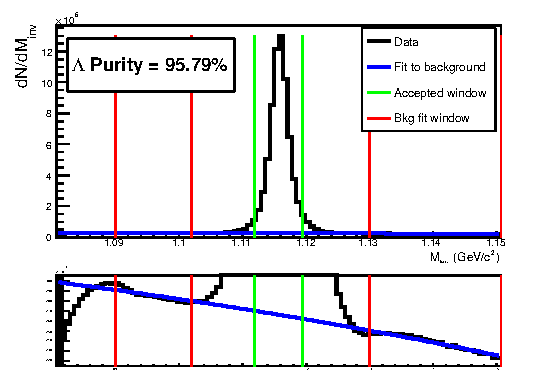
\includegraphics[width=0.49\linewidth]{/home/jesse/Analysis/FemtoAnalysis/LamKPublication/Figures/PDF/LamPurity_LamK0.pdf}}
  %%----start of second subfigure---  
  \subfigure[$\pi^{+}\pi^{-}$ invariant mass distribution where the \Ks peak is seen.]{
    \label{fig:Purity:b}
    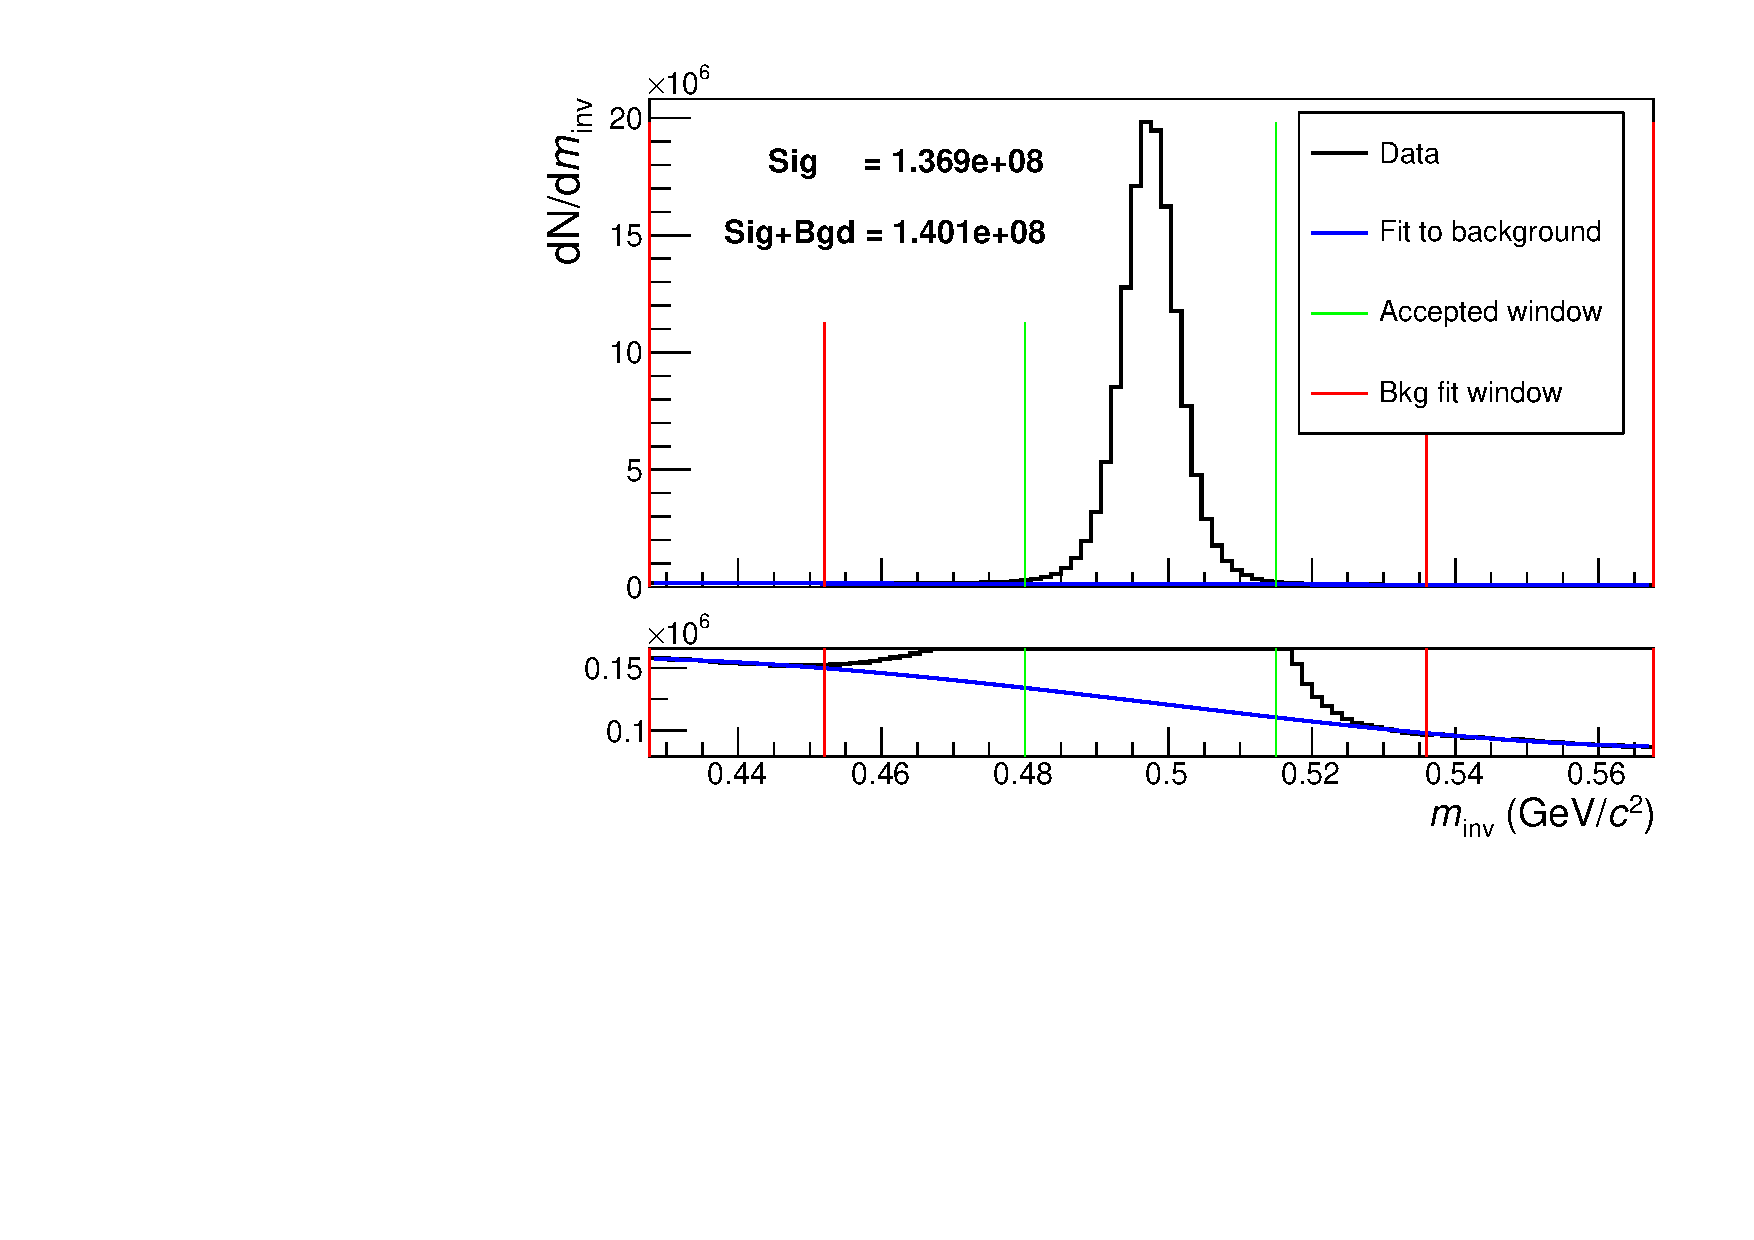
\includegraphics[width=0.49\linewidth]{/home/jesse/Analysis/FemtoAnalysis/LamKPublication/Figures/PDF/K0Purity_LamK0.pdf}}
  %%----overall caption----
  \caption{Invariant mass (\minv) distribution of p$\pi^{+}$ pairs showing the \Lam peak \ref{fig:Purity:a}, and of $\pi^{+}\pi^{-}$ pairs showing the \Ks peak \ref{fig:Purity:b}, for V0 candidates immediately before the final invariant mass cut (for the 0-10\% centrality bin).  The bottom figures are zoomed to show the background with fit.  The vertical green lines represent the \minv cuts used in the analyses, the red vertical lines delineate the region over which the background was fit, and the blue line shows the background fit.  These distributions (or similar, for \ALam) are used to calculate the collection purities, Purity(\Lam) $\approx$ Purity(\ALam) $\approx$ 95\%, and Purity(\Ks) $\approx$ 98\%.}  
  \label{fig:Purity}
\end{figure}






\subsection{Pair Construction}
\label{PairConstruction}
The femtoscopic analysis of two-particle correlation functions relies on the proper formation of particle pairs.
As such, it is important to obtain true particle pairs in the analysis.  
In particular, contamination from pairs constructed with split or merged tracks, and pairs sharing daughters, can introduce an artificial signal into the correlation function, obscuring the actual physics.  
In an effort to remove contamination, we impose two main pair cuts: a shared daughter cut, and an average separation cut.  

The purpose of the shared daughter cut is to ensure the first particle in the pair is unique from the second.  
For pairs formed of two V0s (i.e. \LamKs), this cut is implemented by removing all pairs which share a daughter (ex. in \LamKs analysis, if the \Lam and \Ks in a potential pair claim the same $\pi^{-}$ daughter, the pair is excluded from the analysis).  
For a pair formed of a single V0 and a charged track (i.e. \LamKpm), the cut removes all pairs in which the charged track is also claimed as a daughter of the V0.  
This mistake could only occur if, for instance, a \Kpm is misidentified as a $\pi$ or p either in the V0 reconstruction or in the \Kpm selection.

The purpose of the average separation cut is to remove splitting and merging effects, and it is employed in the following way.  
For each V0-V0 pair (\LamKs), the spatial separation between the same-sign daughters was calculated at several points throughout the TPC (every 20 cm radially from 85 cm to 245 cm), and the results averaged.
Similarly, in the case of a V0-Track pair (\LamKpm), the average separation between the track and the daughter of the V0 sharing the same charge as the track was calculated.
For the \LamALamKs analysis, the average separation for like-charge daughters must be greater than 6.0 cm (we enforce no cut for unlike-charge daughters).  
For example, we impose this cut in a \LamKs analysis on the p daughter of the \Lam and the $\pi^{+}$ daughter of the \Ks.  
For the \LamKpm analyses, the average separation between the \LamALam daughter (sharing the same charge as the \Kpm) and the \Kpm is 8.0 cm (we enforce no cut for unlike signs).  
For a \LamKchP analysis, we impose this cut between the p daughter of the \Lam and the \KchP in the pair.
These cut values were obtained by first forming average separation correlation functions.
This is done just as for our relative-momentum correlation functions, but we instead bin in average separation.
Looking at these average separation correlation functions, at lowest average separation we see an enhancement due to track splitting, followed by a suppression due to track merging.
When the average separation correlation function stabilizes to unity, these effects are no longer abundant, and we choose our cut value.




\section{Analysis Methods}
\label{sec:AnalysisMethods}

\subsection{Correlation Function}
\label{sec:CorrelationFunction}
General remarks about formation of correlation functions and what information they provide.

Two-particle correlation functions are built as the ratio of the covariant two-particle and single-particle spectra:

\begin{equation}
  C^{ab}(\vec{\mathrm{p}_{a}},\vec{\mathrm{p}_{b}}) = \frac{E_{a}E_{b}\frac{dN^{ab}}{d^{3}p_{a}d^{3}p_{b}}}{\big( E_{a}\frac{dN^{a}}{d^{3}p_{a}} \big) \big( E_{b}\frac{dN^{b}}{d^{3}p_{b}} \big)}
\label{eqn:CfRatioSpectra}
\end{equation}

After a few approximations and assumptions, the two-particle relative momentum correlation function (Eq. \ref{eqn:CfRatioSpectra}) may be written as in the Koonin-Pratt equation \cite{Koonin:1977fh, Pratt:1990zq}:

\begin{equation}
 C(\mathbf{k^{*}}) = \int S(\mathbf{r^{*}})|\Psi_{\mathbf{k^{*}}}(\mathbf{r^{*}})|^{2}d^{3}\mathbf{r^{*}}
\label{eqn:KooninPrattEqn}
\end{equation}

where $S(\mathbf{r^{*}})$ is the pair source distribution, $\Psi_{\mathbf{k^{*}}}(\mathbf{r^{*}})$ is the two-particle wave-function, and \kstar is the momentum of one particle in the pair rest frame.
This form emphasizes that $|\Psi|^{2}$ can be considered a kernel with which to transform from a coordinate-space basis to a relative-momentum basis.
This also reveals limitations; distribution of relative positions of particles with identical velocities and total momentum P as they move in asymptotic state.  Therefore, not size of entire source, but "region of homogeneity" [citation Sinyukov].

Within the $|\Psi|^{2}$ term is contained the particle interaction term, allowing us to extract scattering parameters.

In practice, the correlation function is formed experimentally as:

\begin{equation}
  C(k^{*}) = \mathcal{N}\frac{A(k^{*})}{B(k^{*})}
\label{eqn:CfExp}
\end{equation}


where $A(k^{*})$ is the signal distribution, $B(k^{*})$ is the reference (or background) distribution, $\mathcal{N}$ is a normalization parameter, and $k^{*}$ is the momentum of one of the particles in the pair rest frame.  The normalization parameter is chosen such that the mean value of the correlation function equal unity for \kstar $\in$ [0.32, 0.4] GeV/$c$.


In practice, $A(k^{*})$ is constructed by binning in \kstar pairs from the same event.
Ideally, $B(k^{*})$ is similar to $A(k^{*})$ in all respects excluding the presence of femtoscopic correlations \cite{Lisa:2005dd}; as such, $B(k^{*})$ is used to divide out the phase-space effects, leaving only the femtoscopic effects in the correlation function. 
Typically, $B(k^{*})$ is obtained by forming mixed-event pairs, i.e. particles from a given event are paired with particles from $\rm N_{mix}$ other events, and these pairs are then binned in \kstar.
In forming the background distribution, it is important to mix only similar events; mixing events with different phase-spaces can result in an unreliable background distribution, and can introduce artificial signals in the correlation function.
Therefore, in this analysis, we bin our events both in primary vertex location (2 cm bin width) and in centrality (5\% bin width), and we only mix events within a given bin; i.e. we only mix events of like centrality and of like primary vertex location.
Additionally, we use $\rm N_{mix} = 5$ as the size of our mixing pool.
Also note, a vertex correction is also applied to each event, which essentially recenters the the primary vertices to z = 0.

Another option for obtaining the background is to use the Stavinsky method...

This analysis presents correlation functions for three centrality bins (0-10\%, 10-30\%, and 30-50\%), and is currently pair transverse momentum ($k_{\mathrm{T}} = \frac{1}{2}|\mathbf{p}_{\mathrm{T,1}}+\mathbf{p}_{\mathrm{T,2}}|$) integrated (i.e. not binned in $k_{\mathrm{T}}$).  
The correlation functions are constructed separately for the two magnetic field configurations (++ and -~-), and are combined using a weighted average:

\begin{equation}
  C(k^{*}) = \frac{\sum\limits_{i}w_{i}C_{i}(k^{*})}{\sum\limits_{i}w_{i}} 
\label{eqn:CombineCfs}
\end{equation}

where the sum runs over the correlation functions to be combined, and the weight, $w_{i}$, is the number of numerator pairs in the normalization range for $C_{i}(k^{*})$.
In this analysis, the sum is over the two field configurations.


\subsection{Modeling the correlation function}
\label{sec:ModelingCF}


In the absence of Coulomb effects, and assuming a spherically Gaussian source of width $R$, and s-wave scattering, the 1D femtoscopic correlation function can be calculated analytically using \cite{Lednicky:82}:

\begin{equation}
 C(k^{*}) = 1 + C_{QI}(k^{*}) + C_{FSI}(k^{*})
\label{eqn:LednickyEqn}
\end{equation}

$C_{QI}$ describes plane-wave quantum interference:

\begin{equation}
 C_{QI}(k^{*}) = \alpha\exp(-4k^{*2}R^{2})
\label{eqn:CQI}
\end{equation}

where $\alpha = (-1)^{2j}/(2j+1)$ for identical particles with spin j, and $\alpha = 0$ for non-identical particles.  
For all pairs studied in this analysis, $\alpha = 0$.  
$C_{FSI}$ describes the s-wave strong final state interaction between the particles:

\begin{equation}
\begin{array}{l}
\vspace{2mm}  %%space between C_{FSI}(k^{*}) and f(k^{*})
  C_{FSI}(k^{*}) = (1+\alpha)[\frac{1}{2}|\frac{f(k^{*})}{R}|^2(1-\frac{d_{0}}{2\sqrt{\pi}R})+\frac{2\mathbb{R}f(k^{*})}{\sqrt{\pi}R}F_{1}(2k^{*}R)-\frac{\mathbb{I}f(k^{*})}{R}F_{2}(2k^{*}R)] \\
\vspace{2mm}  %%space after f(k^{*})  
  ~~~~~f(k^{*}) = (\frac{1}{f_{0}}+\frac{1}{2}d_{0}k^{*2}-ik^{*})^{-1};~~~
  F_{1}(z) = \int_{0}^{z} \frac{e^{x^{2}-z^{2}}}{z}dx;~~~
  F_{2}(z) = \frac{1-e^{-z^{2}}}{z}
\end{array}  
\label{eqn:CFSI}
\end{equation}

where $R$ is the source size, $f(k^{*})$ is the s-wave scattering amplitude, $f_{0}$ is the complex scattering length, and $d_{0}$ is the effective range of the interaction.

An additional parameter $\lambda$ is typically included in the femtoscopic fit function to account for the purity of the pair sample.  
In the case of no residual correlations (to be discussed in Section \ref{ResidualCorrelations}, the fit function becomes:

\begin{equation}
 C(k^{*}) = 1 + \lambda[C_{QI}(k^{*}) + C_{FSI}(k^{*})]
\label{eqn:LednickyEqnwLambda}
\end{equation}


\subsection{Residual Correlations}
\label{ResidualCorrelations}

The purpose of this analysis is study the interaction and scale of the emitting source of the pairs.
In order to obtain correct results, it is important for our particle collections to consist of primary particles.
In practice, this is difficult to achieve for our \Lam and \ALam collections.
Many of our \Lam particles are not primary, but originate as decay products from other hyperons, including $\Sigma^{0}$, $\Xi^{0}$, $\Xi^{-}$ and $\Sigma^{*(+,-,0)}(1385)$.  
Additionally, many of our K particles are not primary, but decay from K$^{*(+,-,0)}(892)$ parents.
In these decays, the \Lam carries away a momentum very similar to that of its parent.
As a result, the correlation function between a secondary \Lam and, for instance, a \KchP  will be sensitive to, and dependent upon, the interaction between the parent of the \Lam and the \KchP.
In effect, the correlation between the parent of the \Lam and the \KchP (ex. $\Sigma^{0}$\KchP) will be visible, although smeared out, in the \LamKchP data.
We call this a residual correlation resulting from feed-down.  
Residual correlations are important in an analysis when three criteria are met \cite{Kisiel:2014mma}: i) the parent correlation signal is large, ii) a large fraction of pairs in the sample originate from the particular parent system, and iii) the decay momenta are comparable to the expected correlation width in \kstar. 

As it is difficult for us to eliminate these residual correlations in our analyses, we must attempt to account for them in our fit.
The genuine \LamK correlation function may be combined with the contributions from residual feed-down and misidentified particles to obtain the final, measured correlation function:


\begin{eqnarray}
\label{eqn:Residuals} 
 C_{\mathrm{measured}}(k^{*}_{\Lambda\mathrm{K}}) &=& 1 + \lambda'_{\Lambda\mathrm{K}}[C_{\Lambda\mathrm{K}}(k^{*}_{\Lambda\mathrm{K}}) - 1] + \sum\limits_{i,j}  \lambda'_{ij}[C_{ij}(k^{*}_{\Lambda\mathrm{K}})-1] \\
 \lambda_{ij}' &=& \lambda_{\mathrm{Fit}}\lambda_{ij} \notag \\
 \sum\limits_{ij}\lambda_{ij}' &=&  \lambda_{\mathrm{Fit}}\sum\limits_{ij}\lambda_{ij} = \lambda_{\mathrm{Fit}} \notag
\end{eqnarray}

where the \LamK term represents the genuine \LamK correlation, and the $i$, $j$ terms denote the contributions from residual feed-down and possible impurities.
More specifically, $C_{ij}(k^{*}_{\Lambda\mathrm{K}})$ is the correlation function between particles of parent species $i$ and $j$, expressed in the basis of the relative momentum of the observed daughter \LamK pairs.  
The $\lambda$ parameters serve as weight dictating the strength of the parent contribution to the daughter pair, and are normalized to unity.
The individual $\lambda_{ij}$ are fixed (and whose values can be found in Table \ref{tab:LambdaValues_All}), but the parameter $\lambda_{\mathrm{Fit}}$ is left free.
The $\lambda_{\mathrm{Fit}}$ parameter serves as an overall normalization shared by all contributors.

In order to obtain the parent correlation function expressed in the relative momentum of the daughter pair, one must use a transform matrix.
The transform matrix describes the decay kinematics of the parent system into the daughter, and maps the \kstar of the parent pair to that of the daughter.
Using this matrix, the transformed residual correlation function can be obtained:


\begin{equation}
  C_{ij}(k^{*}_{\Lambda\mathrm{K}}) \equiv \frac{\sum\limits_{k^{*}_{ij}} C_{ij}\left(k^{*}_{ij}\right) T\left(k^{*}_{ij},k^{*}_{\Lambda\mathrm{K}}\right)}{\sum\limits_{k^{*}_{ij}} T\left(k^{*}_{ij},k^{*}_{\Lambda\mathrm{K}}\right)}
\label{eqn:ResidualsTransform}
\end{equation}


This transform matrix is generated with THERMINATOR 2 \cite{Chojnacki:2011hb} simulation, and is formed for a given parent pair, $ij$, by taking all \LamK pairs originating from $ij$, calculating the relative momentum of the parents ($k^{*}_{ij}$) and daughters ($k^{*}_{\Lambda\mathrm{K}}$), and filling a two-dimensional histogram with the values. 
The transform matrix is essentially an unnormalized probability distribution mapping the \kstar of the parent pair to that of the daughter pair when one or both parents decay.


For this analysis, the $\lambda$ parameters can be estimated from simulation.  
The reconstruction efficiency for primary \Lam particles is nearly equal to that of \Lam particles originating from $\Sigma$, $\Sigma^{*}$, $\Xi^{0}$, $\Xi^{-}$, and $\Omega$ hyperons \cite{Salzwedel:2241303}.  
Therefore, the $\lambda$ parameter for parent system $ij$ can be estimated using THERMINATOR 2 as the total number of \LamK pairs originating from $ij$ ($\mathrm{N}_{ij}$) divided by the total number of \LamK pairs ($\rm N_{Total}$): 

\begin{equation}
\lambda_{ij} = \frac{\mathrm{N}_{ij}}{\mathrm{N_{Total}}}
\end{equation}

The $\lambda$ parameters used for this study can be found in Tab. \ref{tab:LambdaValues_All} in Appendix \ref{App:LamParams}.

Now, on to the question of how we model the parent correlation functions, $C_{ij}$.  
In an ideal world, we would simply look up the parent interaction in some table, and input this into our model.  
Unfortunately, the world in which we live is not perfect, such a table does not exists, and little is know about the interaction between the particles in the residual pairs of this study. 
Additionally, introducing a unique set of scattering parameters and radii for each residual system would introduce a large number of additional fit parameters, for which we do not have many constraints, and would cause our fitter to be too unconstrained and yield untrustworthy results. 
For this analysis, we assume all residual pairs have the same source size as the daughter pair.
Furthermore, we assume Coulomb-neutral residual pairs share the same scattering parameters as the daughter pair.
Therefore, for Coulomb-neutral pairs, such as \LamK, $\Sigma^{0}$K, and $\Xi^{0}$K, $C_{ij}(k^{*}_{ij})$ is calculated from Eqn. \ref{eqn:LednickyEqn}, with the help of Eqn. \ref{eqn:CFSI}; $C_{ij}(k^{*}_{\Lambda\mathrm{K}})$ is then obtained by transforming $C_{ij}(k^{*}_{ij})$ with Eq. \ref{eqn:ResidualsTransform}.  

For residual pairs affected by both the strong and Coulomb interactions, things are a bit more complicated.
This is due to the fact that, for the case of both strong and Coulomb interaction, we no longer have a nice analytical form with which to fit.
Generating a correlation function including both is also time consuming, as described further in Appendix \ref{App:CoulombFitter}.
Therefore, to treat this case, we have two different methods.
First, we can use our experimental \XiKpm data to represent the charged parent pair system.  
Alternatively, we can assume the strong interaction is negligible in the charged residual, and generate the parent correlation function given radius and $\lambda$ parameters (see Appendix \ref{App:CoulombFitter} for more details).  
We find in our \XiKpm study that a Coulomb-only description of the system describes, reasonably well, the broad features of the correlation.  
The strong interaction is necessary for the fine details.  
However, as these correlations are run through a transform matrix, which largely flattens out and fine details, a Coulomb-only description should be sufficient.  
We find consistent results between using the $\Xi$K data and the Coulomb-only interpolation method. 
When modeling \XiKpm residual correlations, we use the experimental \XiKpm data; in this case, there is no need to make any assumptions about scattering parameters or source sizes, as we already have the experimental data.  
When the number of residual pairs used is increased to 10, so that additional charged residual pairs such as $\Sigma^{*+}$K$^{-}$ enter the picture, the Coulomb-only interpolation method is used.


\subsection{Momentum Resolution Corrections}
\label{MomentumResolutionCorrections}

Finite track momentum resolution causes the reconstructed momentum of a particle to smear around the true value.
This, of course, also holds true for V0 particles.
The effect is propagated up to the pairs of interest, which causes the reconstructed relative momentum (\krec) to differ from the true momentum (\ktrue).
Smearing of the momentum typically will result in a suppression of the signal.

The effect of finite momentum resolution can be investigated using the MC data, for which both the true and reconstructed momenta are available.

Information gained from looking at \krec vs \ktrue can be used to apply corrections to account for the effects of finite momentum resolution on the correlation functions.



A second approach is to use information gained from response matrices.
The response matrix describes quantitatively how each \krec bin receives contributions from multiple \ktrue bins, and can be used to account for the effects of finite momentum resolution.
With this approach, the resolution correction is applied on-the-fly during the fitting process by propagating the theoretical (fit) correlation function through the response matrix, according to:  

\begin{equation}
  C_{\mathrm{fit}}(k^{*}_{\mathrm{Rec}}) = \dfrac{\sum\limits_{k^{*}_{\mathrm{True}}}M_{k^{*}_{\mathrm{Rec}},k^{*}_{\mathrm{True}}}C_{\mathrm{fit}}(k^{*}_{\mathrm{True}})}{\sum\limits_{k^{*}_{\mathrm{True}}}M_{k^{*}_{\mathrm{Rec}},k^{*}_{\mathrm{True}}}}
\label{eqn:MomResCorrection}
\end{equation}

where $M_{k^{*}_{\mathrm{Rec}},k^{*}_{\mathrm{True}}}$ is the response matrix, $C_{\mathrm{fit}}(k^{*}_{\mathrm{True}})$ is the fit binned in \ktrue, and the denominator normalizes the result.

Equation \ref{eqn:MomResCorrection} describes that, for a given \krec bin, the observed value of $C(k^{*}_{\mathrm{Rec}})$ is a weighted average of all $C(k^{*}_{\mathrm{True}})$ values, where the weights are the normalized number of counts in the [\krec, \ktrue] bin.



\subsection{Non-Flat Background}
\label{NonFlatBackground}

We observe a significant non-femtoscopic, non-flat, background in all of our correlations at large \kstar.  
This background increases with decreasing centrality, is the same amongst all \LamKpm pairs, and is more pronounced in the \LamKs system.
This difference in \LamKpm and \LamKs backgrounds is due mainly to the difference in kinematic cuts, not due to any interesting physics.  


It is suggested that this background effect is due primarily to particle collimation associated with elliptic flow \cite{Kisiel:2017}.  
More specifically, these backgrounds result from mixing events with unlike event-plane angles ($\Psi_{\textrm{EP}}$).  
As explained in \cite{Kisiel:2017}, when elliptic flow is present, all particles are more likely to be emitted in a specific direction (in-plane), as opposed to a perpendicular direction.  
Therefore, the difference in momenta for pairs of particles tends to be smaller, compared to the case of no flow.  
In the case of mixed-event pairs, the two events used do not share an event-plane, and therefore there is no collimation effect in the pairs from flow.  
As a result, pairs with larger momentum are more likely when mixed-events are used, causing the correlation function to be observed below unity.  
In general, a dip below unity, at a given \kstar, means it is more probable to find a pair at that \kstar when the daughters are taken from mixed-events, as compared to when they are taken from the same event.

This same reasoning suggests that the background should lead to an enhancement at low-\kstar.  
The enhancement at high-\kstar (\kstar $\gtrsim$ 1.5 GeV/$c$) does not result from the collective flow of the system.  
We are not certain was causes this enhancement, but typical suspects are jet-like correlations and resonance decays.



THERMINATOR 2 simulation has been shown to reproduce the background features in a $\pi$K analysis \cite{Kisiel:2017}.  
As the background effect can be attributed mainly to elliptic flow, which is a global feature of the system, we suspected THERMINATOR 2 could also, at least qualitatively, describe our backgrounds.  
After ensuring each simulated event received a random event-plane angle ($\Psi_{\mathrm{EP}}$), we found THERMINATOR 2 did a good job of describing our data qualitatively, and, in many cases, quantitatively.  

\subsection{LednickyFitter}
\label{LednickyFitter}


A simple $\chi^{2}$ test is inappropriate for fitting correlation functions, as the ratio two Poisson distributions does not result in a Poisson distribution.
Instead, a log-likelihood fit function of the following form is used \cite{Lisa:2005dd}:

\begin{equation}
 \chi^{2}_{PML} = -2\left[A\ln\left(\frac{C(A+B)}{A(C+1)}\right) + B\ln\left(\frac{A+B}{B(C+1)}\right)\right]
\label{eqn:Chi2PML}
\end{equation}

where $A$ is the experimental signal distribution (numerator), $B$ is the experimental background distribution (denominator), and $C$ is the theoretical fit correlation function.

The fitter uses Equations \ref{eqn:LednickyEqn} -- \ref{eqn:CFSI} to build the theoretical fit, and Equation \ref{eqn:Chi2PML} as the statistic quantifying the quality of the fit.
The parameters of the fit are: $\lambda$, $R$, $f_{0}$ ($\mathbb{R}f_{0}$ and $\mathbb{I}f_{0}$ separately), $d_{0}$, and normalization $N$.
The fitter currently includes methods to correct for momentum resolution and a non-flat background.
These corrections are applied to the fit function, the data is never touched.
The fitter is able to share parameters between different analyses and fit all simultaneously.  

In a typical fit, a given pair is fit with its conjugate (ex. \LamKchP with \ALamKchM) across all centralities (0-10\%, 10-30\%, 30-50\%), for a total of 6 simultaneous analyses.
Each analysis has a unique $\lambda$ and normalization parameter.
The radii are shared between analyses of like centrality, as these should have similar source sizes.
The scattering parameters ($\mathbb{R}f_{0}$, $\mathbb{I}f_{0}$, $d_{0}$) are shared amongst all.

To summarize, the complete fit function is constructed as follows:

\begin{enumerate}
 \item The uncorrected, primary, correlation function, $C_{\Lambda\mathrm{K}}$(\ktrue), is constructed using Eqns. \ref{eqn:LednickyEqn} and \ref{eqn:CFSI}
 \item If residuals are included:
 \begin{itemize}
  \item the parent correlation functions are obtained using:
  \begin{itemize}
   \item Eqns. \ref{eqn:LednickyEqn} and \ref{eqn:CFSI} for the case of Coulomb-neutral pairs
   \item \XiKpm experimental data for \XiKpm contributions
   \item a Coulomb-only curve, with the help of Appendix \ref{App:CoulombFitter}, for pairs including the Coulomb interaction 
  \end{itemize} 
 \item the contribution to the \LamK correlation function is found by running the parent correlation function through the appropriate transform, via Eq.\ref{eqn:ResidualsTransform} 
 \end{itemize} 
 \item The primary and residual correlations are combined, via Eq.\ref{eqn:Residuals}, to form $C'_{Fit}$(\ktrue)
 \begin{itemize}
  \item in the case of no residual contributions included in the fit, $\lambda_{i}$ = $\lambda_{\Lambda\mathrm{K}}$ in Eq. \ref{eqn:Residuals} is set equal to 1.  Then, the extracted $\lambda_{\mathrm{Fit}}$ parameter should be roughly equal to the pair purity
  \item when residuals are included, the $\lambda_{i}$ values are presented in Table \ref{tab:LambdaValues_All}
 \end{itemize} 
 \item The correlation function is corrected to account for momentum resolution effects using Eq. \ref{eqn:MomResCorrection}
 \begin{itemize}
  \item $C'_{\mathrm{Fit}}(k^{*}_{\mathrm{Rec}}) = \dfrac{\sum\limits_{k^{*}_{\mathrm{True}}}M_{k^{*}_{\mathrm{Rec}},k^{*}_{\mathrm{True}}}C'_{\mathrm{Fit}}(k^{*}_{\mathrm{True}})}{\sum\limits_{k^{*}_{\mathrm{True}}}M_{k^{*}_{\mathrm{Rec}},k^{*}_{\mathrm{True}}}}$
 \end{itemize}
 \item Finally, the non-flat background correction is applied, and the final fit function is obtained
 \begin{itemize}
  \item $C_{\mathrm{Fit}}(k^{*}_{\mathrm{Rec}}) = C'_{\mathrm{Fit}}(k^{*}_{\mathrm{Rec}})*F_{\mathrm{Bgd}}(k^{*}_{\mathrm{Rec}})$
 \end{itemize}
\end{enumerate}

\subsection{Systematic uncertainties}
\label{SysErrs}

In order to understand my systematic uncertainties, the analysis code was run many times using slightly different values for a number of important cuts, and the results were compared.

In order to quantify the systematic errors on the data, all correlation functions built using all varied cut values were bin-by-bin averaged, and the resulting variance of each bin was taken as the systematic error.  
The cuts which were utilized in this study are presented in Sections \ref{SysErrsLamK0:ParticleAndPairCuts} (\LamKs) and \ref{SysErrsLamKch:ParticleAndPairCuts} (\LamKpm).


Similarly, the fit parameters extracted from all of these correlation functions were averaged, and the resulting variances were taken as the systematic errors for the fit parameters.
As with the systematic errors on the data, this was performed for all varied cut values.
Additionally, a systematic analysis was done on our fit method.
These two sources of uncertainty were combined in quadrature to obtain the final systematic uncertainties on the extracted fit parameters.

The cuts included in the systematic study, as well as the values used in the variations, are shown in Tab. \ref{tab:LamK0sSystematics} (\LamKs) and Tab. \ref{tab:LamKchSystematics} (\LamKpm).  
Note, the central value corresponds to that used in the analysis.

We fit our non-flat background with a linear function.  
To study the contribution of this choice to our systematic errors, we also fit with a quadratic and Gaussian form. 
The resulting uncertainties are combined with the uncertainties arising from our particle cuts.

Our choice of \kstar fit range was varied by $\pm$ 25\%.  
The resulting uncertainties in the extracted parameter sets were combined with our uncertainties arising from our particle and pair cuts.

\begin{table}[htbp]
 \centering 
  \renewcommand{\arraystretch}{1.2}
  \begin{tabular}{c|c}
   \multicolumn{2}{c}{\LamKs systematics} \\
   \hline  
   DCA \LamALam & 4, 5, 6 mm \\
   \hline
   DCA \Ks & 2, 3, 4 mm \\
   \hline
   DCA \LamALam Daughters & 3, 4, 5 mm \\
   \hline
   DCA \Ks Daughters & 2, 3, 4 mm \\
   \hline
   \LamALam Cosine of Pointing Angle & 0.9992, 0.9993, 0.9994 \\
   \hline
   \Ks Cosine of Pointing Angle & 0.9992, 0.9993, 0.9994 \\
   \hline
   DCA to Primary Vertex of p($\bar{\mathrm{p}}$) Daughter of \LamALam & 0.5, 1, 2 mm \\
   \hline
   DCA to Primary Vertex of $\pi^{-}$($\pi^{+}$) Daughter of \LamALam &  2, 3, 4 mm \\ 
   \hline
   DCA to Primary Vertex of $\pi^{+}$ Daughter of \Ks & 2, 3, 4 mm \\
   \hline
   DCA to Primary Vertex of $\pi^{-}$ Daughter of \Ks & 2, 3, 4 mm \\
   \hline
   Average Separation of Like-Charge Daughters & 5, 6, 7 cm \\
   \hline
  \end{tabular}
 \caption{\LamKs systematics}
 \label{tab:LamK0sSystematics} 
\end{table}


\begin{table}[htbp]
 \centering 
  \renewcommand{\arraystretch}{1.2}
  \begin{tabular}{c|c}
   \multicolumn{2}{c}{\LamKpm systematics} \\
   \hline  
   DCA \LamALam & 4, 5, 6 mm \\
   \hline
   DCA \LamALam Daughters & 3, 4, 5 mm \\
   \hline
   \LamALam Cosine of Pointing Angle & 0.9992, 0.9993, 0.9994 \\
   \hline
   DCA to Primary Vertex of p($\bar{\mathrm{p}}$) Daughter of \LamALam &  0.5, 1, 2 mm \\
   \hline
   DCA to Primary Vertex of $\pi^{-}$($\pi^{+}$) Daughter of \LamALam &  2, 3, 4 mm  \\
   \hline
   Average Separation of \LamALam Daughter with Same Charge as \Kpm & 7, 8, 9 cm \\
   \hline
   Max. DCA to Primary Vertex in Transverse Plane of \Kpm & 1.92, 2.4, 2.88 \\
   \hline
   Max. DCA to Primary Vertex in Longitudinal Direction of \Kpm & 2.4, 3.0, 3.6 \\
   \hline
  \end{tabular}
 \caption{\LamKpm systematics}
 \label{tab:LamKchSystematics} 
\end{table}







\section{Results}
\label{sec:Results}

Figure \ref{fig:LamKFits_3Res} shows fits, with 3 residual correlations included, for all \LamK analyses across all studied centralities (0-10\%, 10-30\%, and 30-50\%).
For the \LamKs results, all analyses are fit simultaneously across all centralities.
A single $\lambda$ parameter is shared amongst all.
Each analysis has a unique normalization parameter.
The radii are shared between analyses of like centrality.
The scattering parameters ($\mathbb{R}f_{0}$, $\mathbb{I}f_{0}$, $d_{0}$) are shared amongst all.
For the \LamKpm results, all analyses are fit simultaneously across all centralities.
Scattering parameters ($\mathbb{R}f_{0}$, $\mathbb{I}f_{0}$, $d_{0}$) are shared between pair-conjugate systems (i.e. a parameter set describing the \LamKchP \& \ALamKchM system, and a separate set describing the \LamKchM \& \ALamKchP system).
For each centrality, a radius and $\lambda$ parameters are shared between all pairs (\LamKchP, \ALamKchM, \LamKchM, \ALamKchP).
Each analysis has a unique normalization parameter.

\begin{figure}[htp]
  \centering
  %%----start of first subfigure---
  \subfigure[\LamKchPALamKchM]{
    \label{fig:LamKFits_3Res:a}
    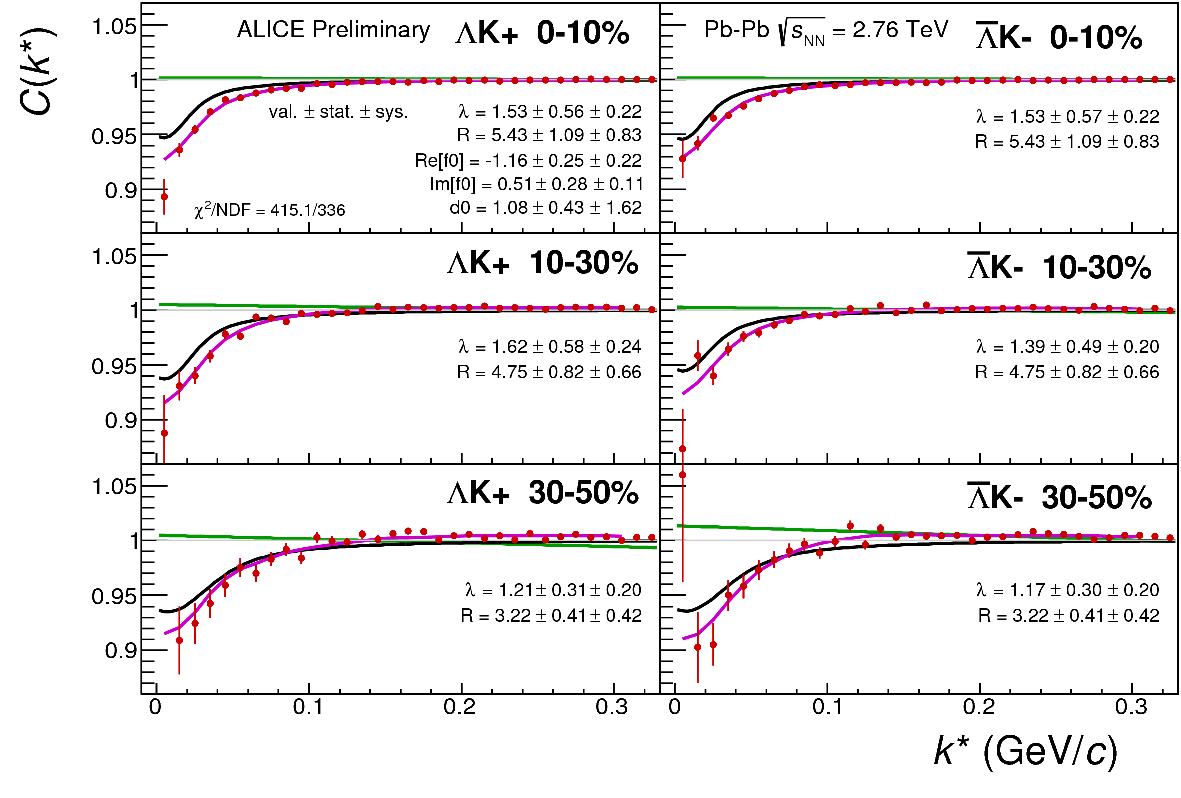
\includegraphics[width=0.49\linewidth]{/home/jesse/Analysis/FemtoAnalysis/LamKPublication/Figures/20171227/PDF/canKStarCfwFitsLamKchPwConj_0010_1030_3050_MomResCrctn_NonFlatBgdCrctn_3Res_PrimMaxDecay4fm_UsingXiDataAndCoulombOnly.pdf}}
  %%----start of second subfigure---  
  \subfigure[\LamKchMALamKchP]{
    \label{fig:LamKFits_3Res:b}
    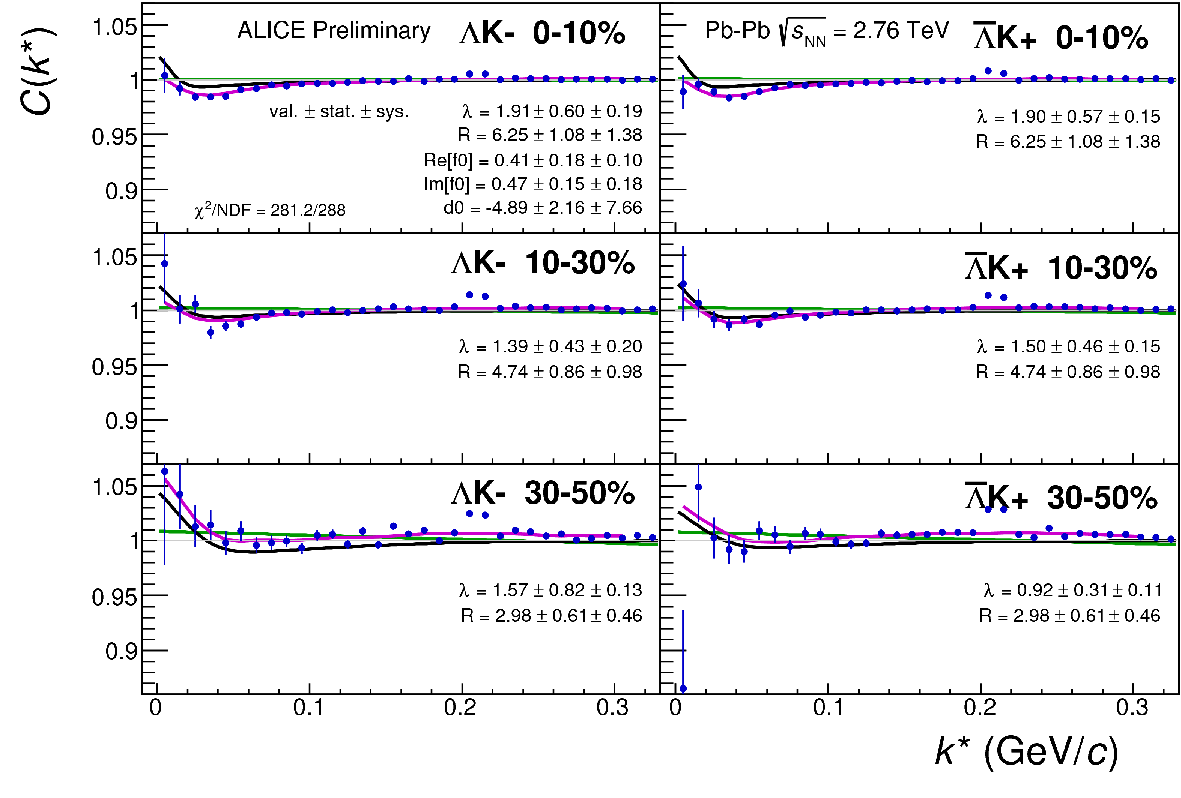
\includegraphics[width=0.49\linewidth]{/home/jesse/Analysis/FemtoAnalysis/LamKPublication/Figures/20171227/PDF/canKStarCfwFitsLamKchMwConj_0010_1030_3050_MomResCrctn_NonFlatBgdCrctn_3Res_PrimMaxDecay4fm_UsingXiDataAndCoulombOnly.pdf}}
  \\  
  %%----start of third subfigure---  
  \subfigure[\LamKsALamKs]{
    \label{fig:LamKFits_3Res:c}
    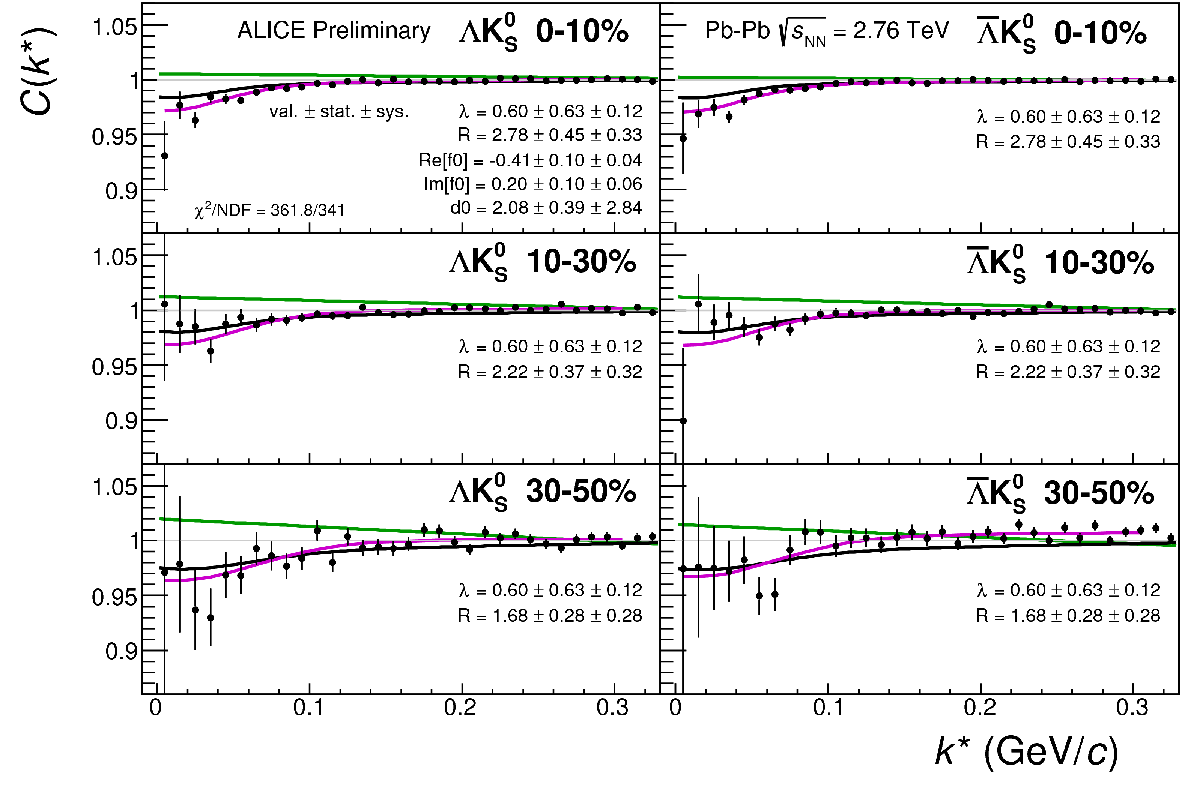
\includegraphics[width=0.49\linewidth]{/home/jesse/Analysis/FemtoAnalysis/LamKPublication/Figures/20171227/PDF/canKStarCfwFitsLamK0wConj_0010_1030_3050_MomResCrctn_NonFlatBgdCrctn_SingleLamParam_3Res_PrimMaxDecay4fm_UsingXiDataAndCoulombOnly.pdf}}    
  %%----overall caption----
  \caption{Fits, with 3 residual correlations included, for all \LamK analyses across all studied centralities (0-10\%, 10-30\%, and 30-50\%).
 The lines represent the statistical errors, while the boxes represent the systematic errors.
 The backgrounds are modeled by (6$^{\mathrm{th}}$-)degree polynomials fit to THERMINATOR simulation.
 The black solid line represents the primary (\LamK) correlation's contribution to the fit.  
 The green line shows the fit to the non-flat background.
 The purple points show the fit after all residuals' contributions have been included, and momentum resolution and non-flat background corrections have been applied.
 The extracted fit values with uncertainties are printed.}  
  \label{fig:LamKFits_3Res}
\end{figure}

\begin{figure}[h]
  \centering
  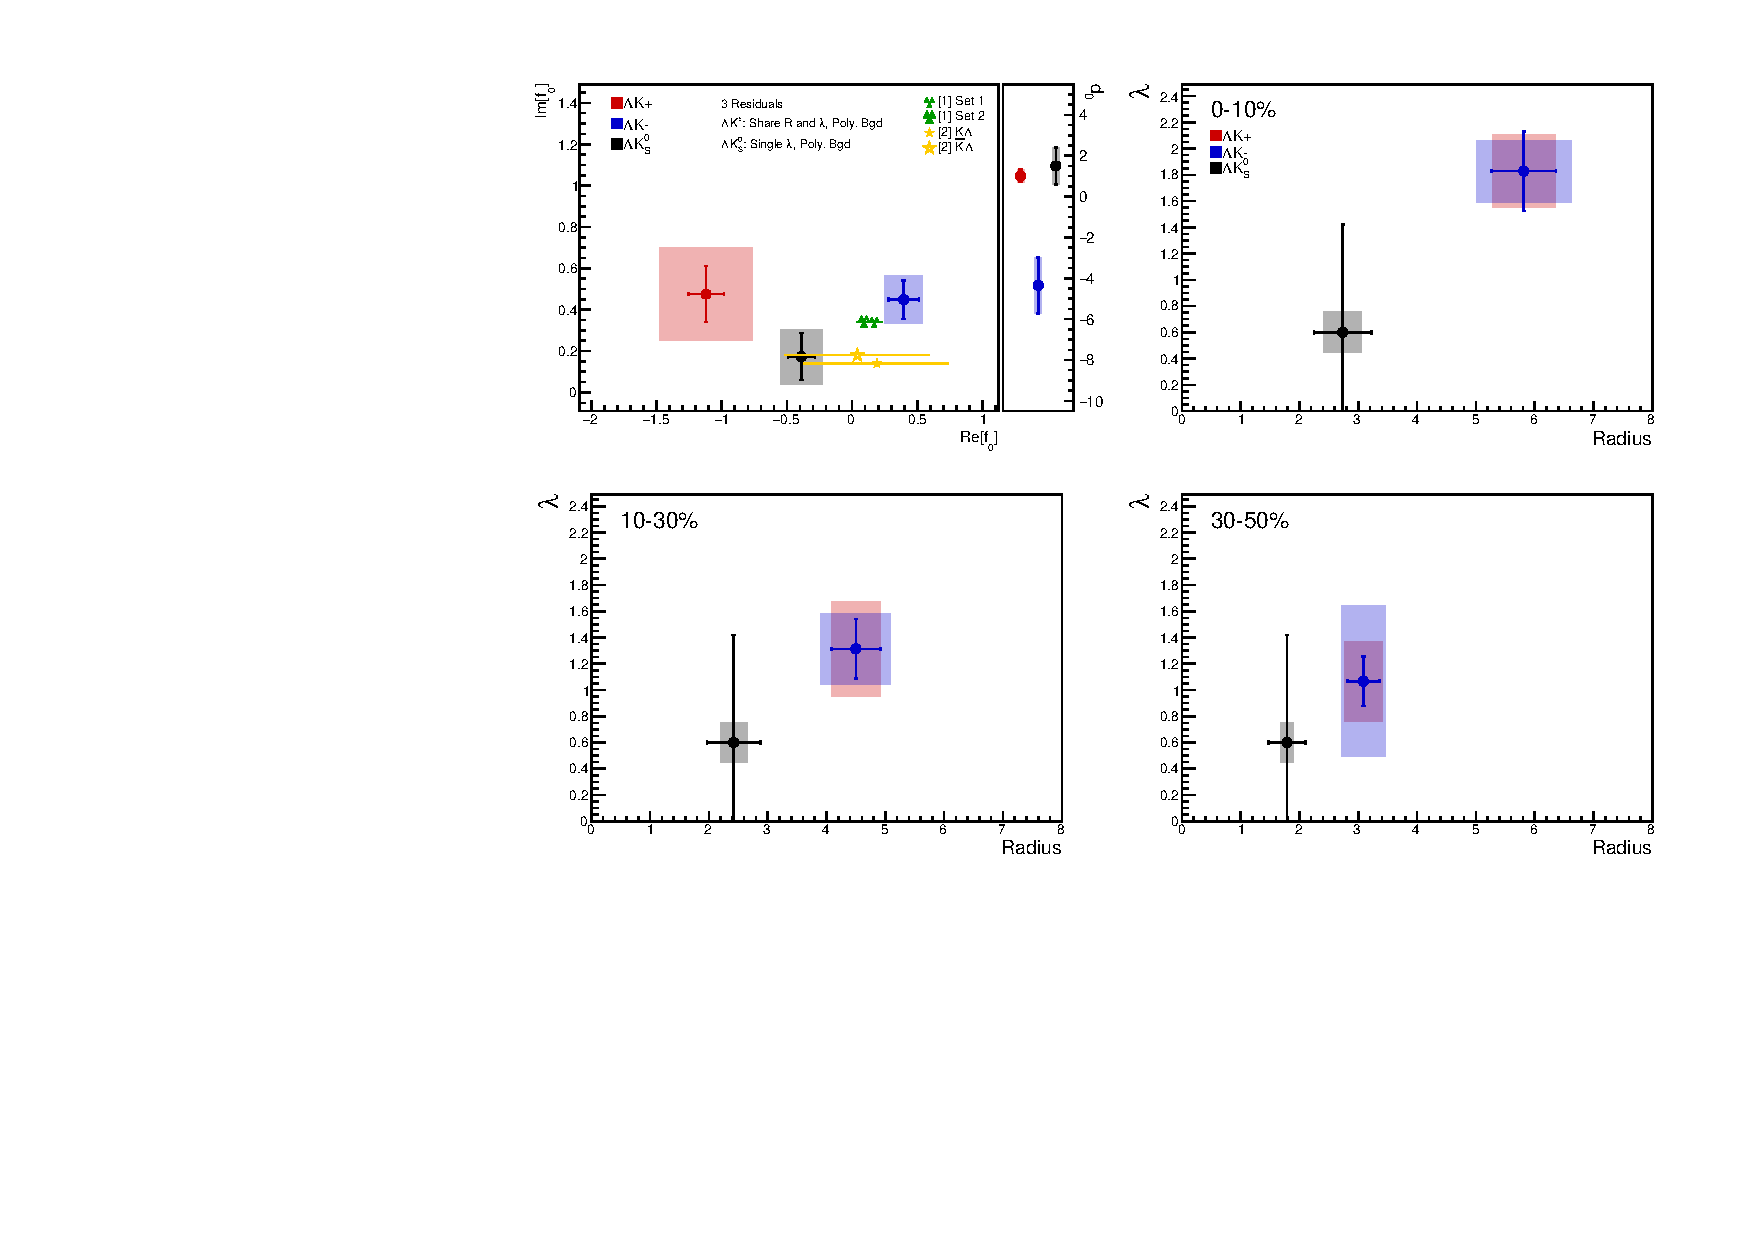
\includegraphics[width=0.80\textwidth]{/home/jesse/Analysis/FemtoAnalysis/AnalysisNotes/7_ResultsAndDiscussion/Figures/CompareAllScattParams_Comp3An_3Res.pdf}
  \caption[Extracted Scattering Parameters: 3 Residuals in Fit]{Extracted scattering parameters for the case of 3 residual contributors for all of our $\Lambda$K systems.  [Top Left]: $\mathbb{I}f_{0}$ vs. $\mathbb{R}f_{0}$, together with d$_{0}$ to the right.  [Top Right (Bottom Left, Bottom Right)]: $\lambda$ vs. Radius for the 0-10\% (10-30\%, 30-50\%) bin.  The green \cite{Liu:2006xja} and yellow \cite{Mai:2009ce} points show theoretical predictions made using chiral perturbation theory.}
  \label{fig:ScattParams_3Res}
\end{figure}

\begin{figure}[h]
  \centering
  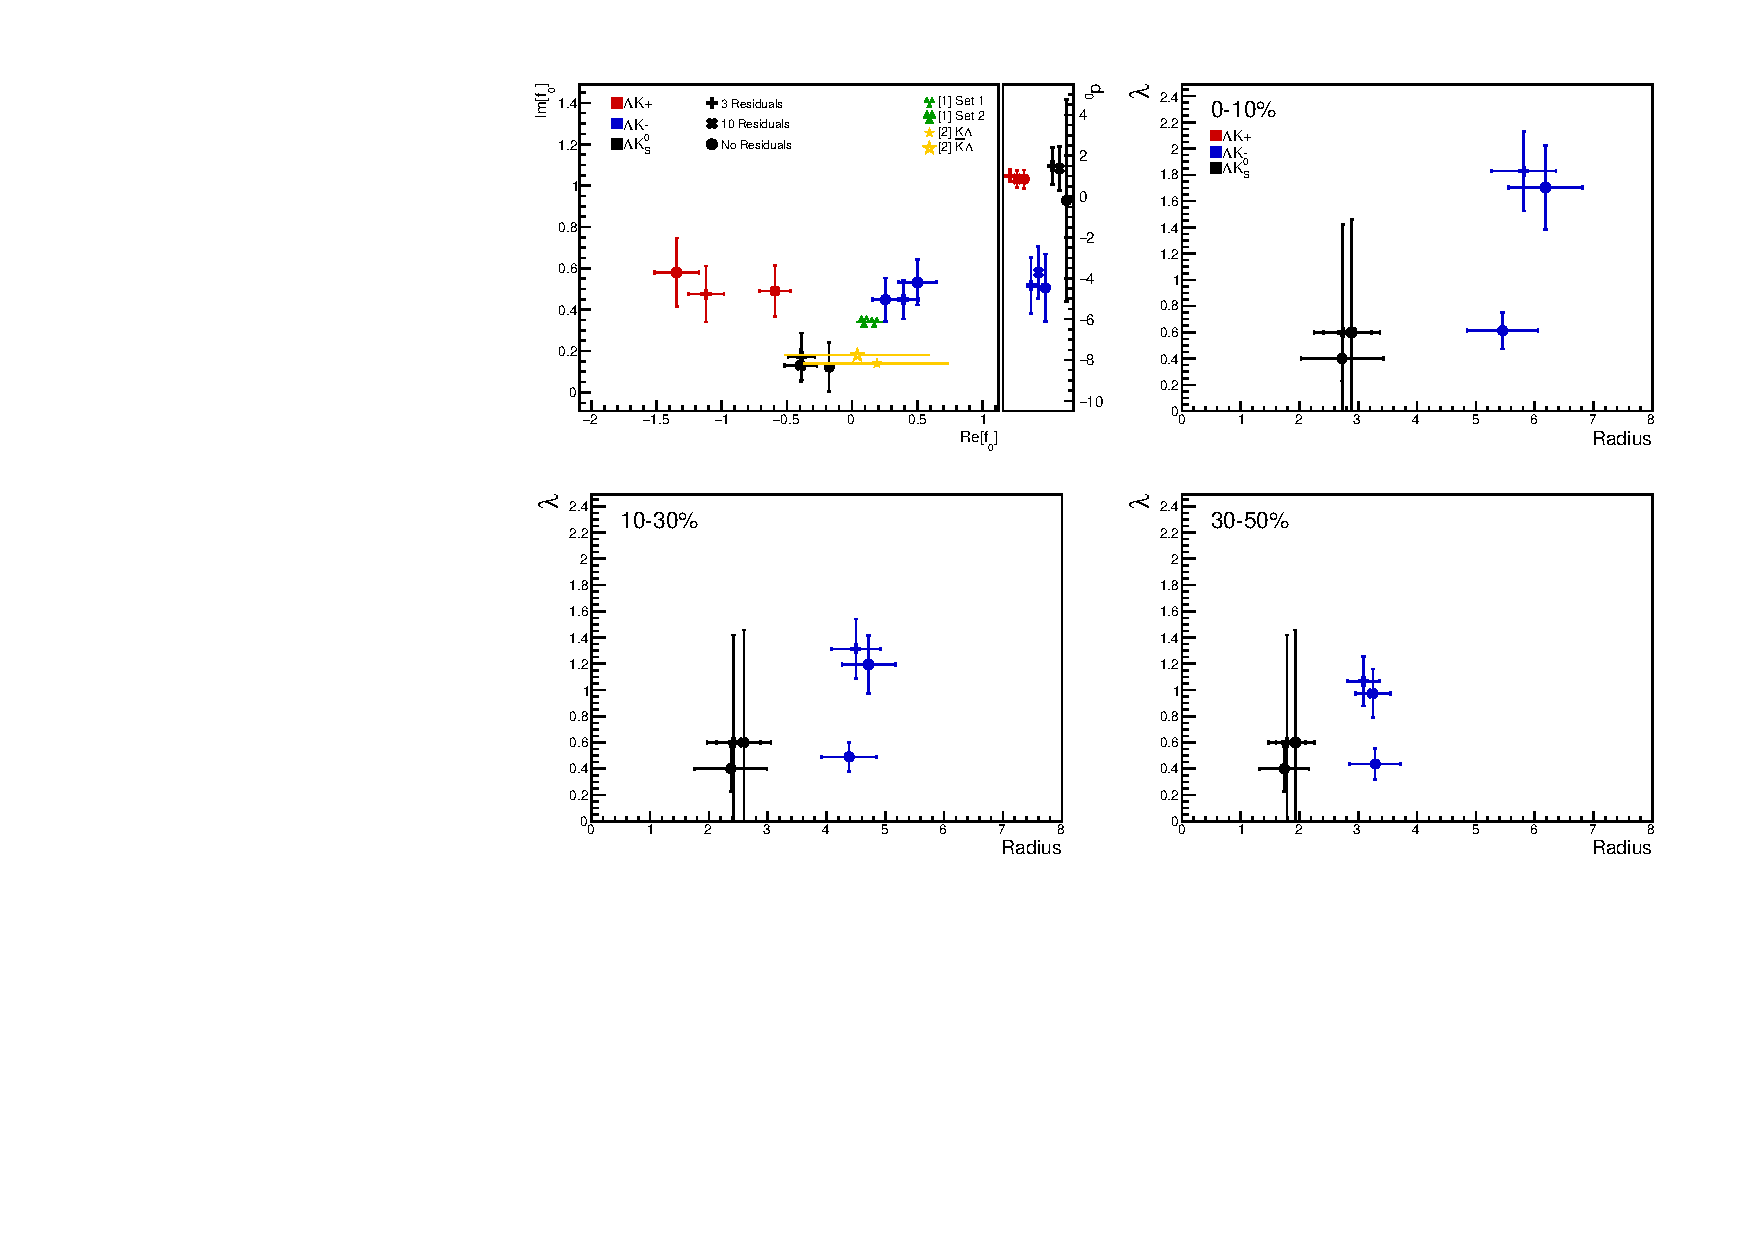
\includegraphics[width=\textwidth]{/home/jesse/Analysis/FemtoAnalysis/AnalysisNotes/7_ResultsAndDiscussion/Figures/CompareAllScattParams_CompNumRes_StatOnly.pdf}
  \caption[Compare Fit Parameters: Number of residuals]{Compare Fit Parameters: Number of residuals: Results shown for the case of 3 (+), 10 (X), and no (circles) residual contributors.}
  \label{fig:CompareAllScattParams_CompNumRes}
\end{figure}


\begin{figure}[h]
  \centering
  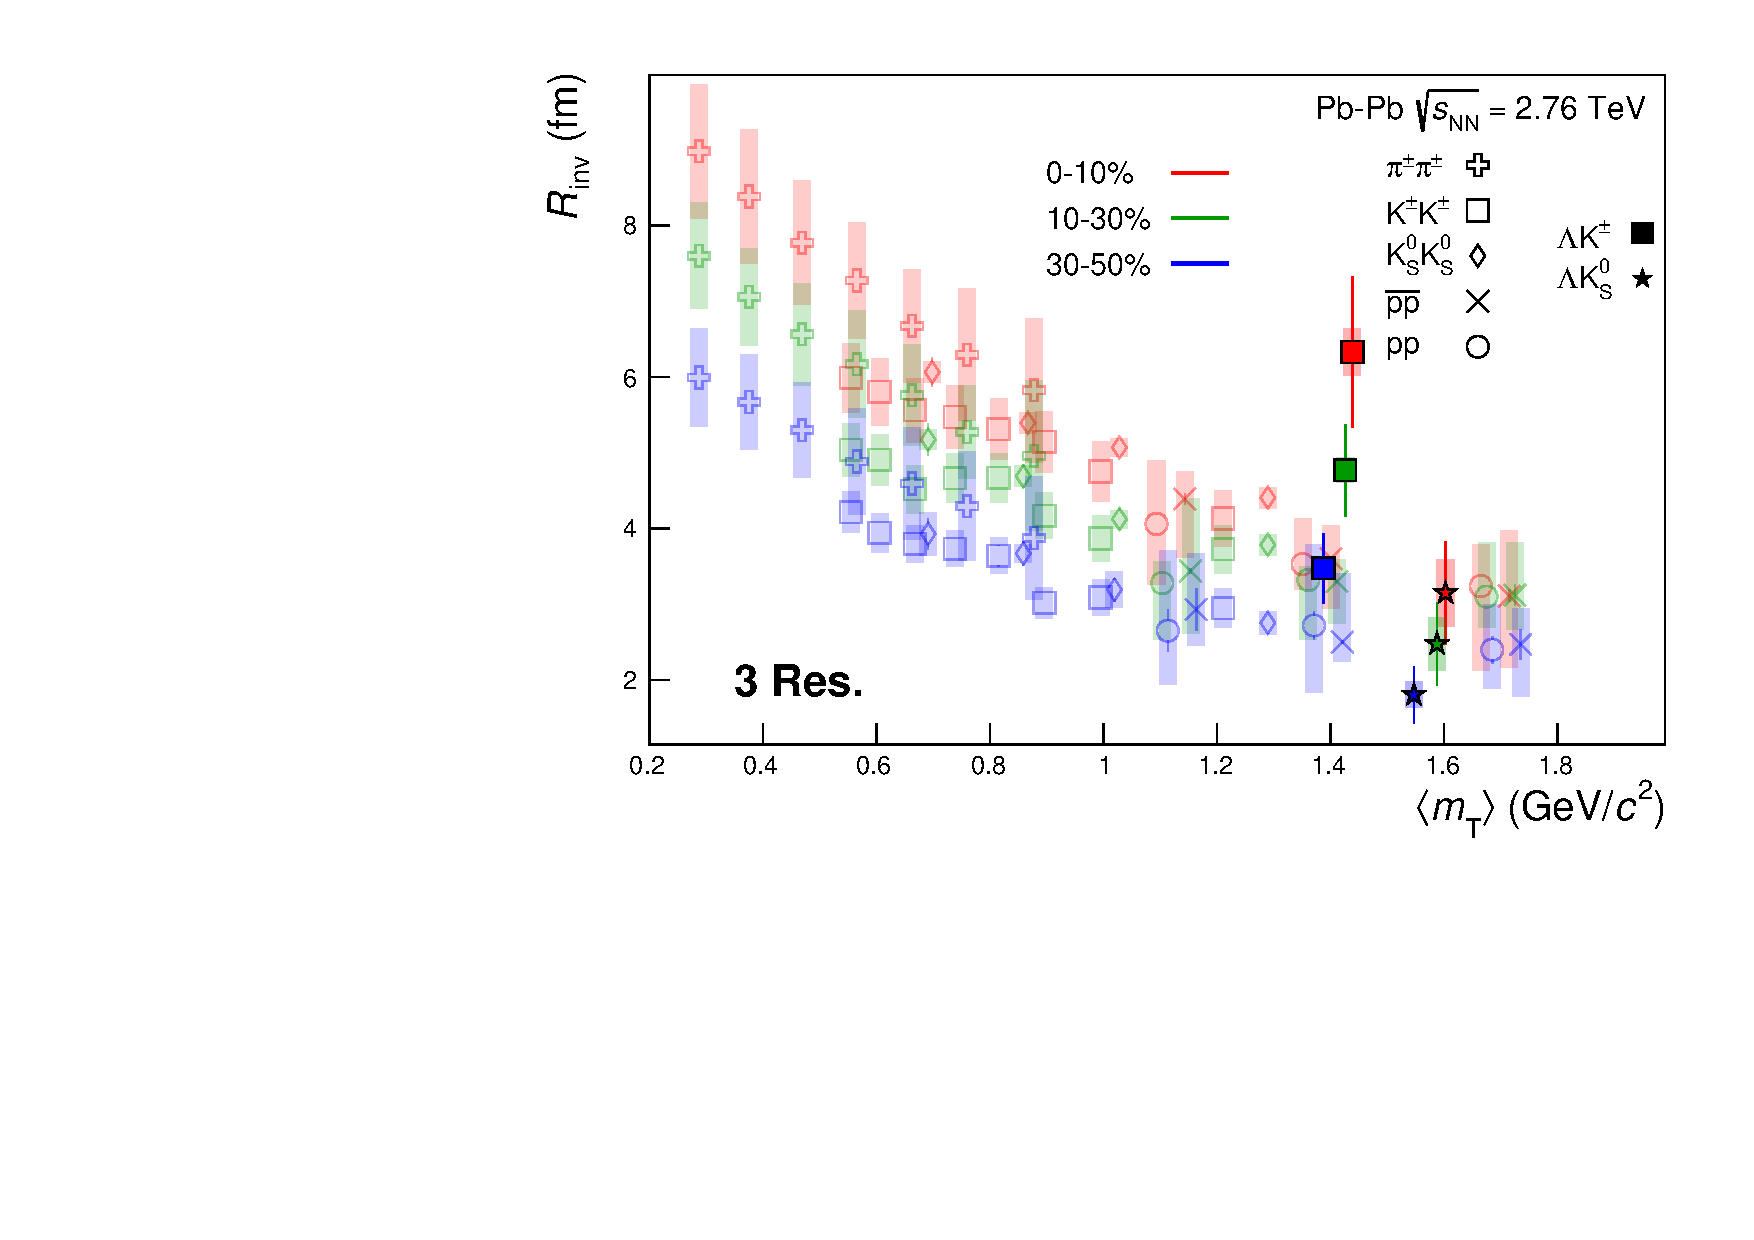
\includegraphics[width=0.5\textwidth]{/home/jesse/Analysis/FemtoAnalysis/AnalysisNotes/7_ResultsAndDiscussion/Figures/mTscaling_MinvCalc_OutlinedPoints_OthersTransparent_3Res.pdf}
  \caption[\mt Scaling of Radii: 3 Residuals in Fit]{3 residual correlations in \LamK fits.  Extracted fit $R_{\mathrm{inv}}$ parameters as a function of pair transverse mass (\mt) for various pair systems over several centralities. The ALICE published data \cite{Adam:2015vja} is shown with transparent, open symbols.  The new \LamK results are shown with opaque, filled symbols.  In the left, the \LamKchP (with it's conjugate pair) results are shown separately from the \LamKchM (with it's conjugate pair) results.  In the right, all \LamKpm results are averaged.}
  \label{fig:mTScalingOfRadii_3Res}
\end{figure}




\section{Summary}
\label{sec:Summary}
We did physics, and we found physics.
But, most importantly, in the end, physics found us.

\clearpage

%%%%% acknowledgements
\newenvironment{acknowledgement}{\relax}{\relax}
\begin{acknowledgement}
\section*{Acknowledgements}
%\input{acknowledgements.tex}    %%%%%%% done by webmaster team
\end{acknowledgement}

%%%%%%%% Bibliography (In case of using bibtex generate the bbl requested by arXiv)
\bibliographystyle{utphys}   % Remember we use title in the biblio
\bibliography{LamK_bibfile}
%\input {bibliography.tex}  

%%%%%%%%% appendix with author list
\newpage
\appendix
%
%\input{}               %%%%%%%%%%% put your appendices here
%


\pagestyle{empty}
\begin{landscape}

\section{$\lambda$ Parameters}
\label{App:LamParams}

\begin{table}[htbp]
 \centering
 \renewcommand{\arraystretch}{1.2}
 \resizebox{\paperwidth}{!}{
 \begin{tabular}{|c|cV{5.0}c|cV{5.0}c|cV{5.0}c|cV{5.0}c|cV{5.0}c|c|}
  \multicolumn{2}{c}{\LamKchP residuals} & \multicolumn{2}{c}{\ALamKchM residuals} & \multicolumn{2}{c}{\LamKchM residuals} & \multicolumn{2}{c}{\ALamKchP residuals} & \multicolumn{2}{c}{\LamKs residuals} & \multicolumn{2}{c}{\ALamKs residuals} \\
  \hline
  \textbf{Pair System} & \textbf{$\lambda$ value} & \textbf{Pair System} & \textbf{$\lambda$ value} & \textbf{Pair System} & \textbf{$\lambda$ value} & \textbf{Pair System} & \textbf{$\lambda$ value} & \textbf{Pair System} & \textbf{$\lambda$ value} & \textbf{Pair System} & \textbf{$\lambda$ value} \\
  \hlineB{3.0}
  \multicolumn{12}{|c|}{3 Residuals} \\
  \hlineB{3.0}
  \LamKchP & 0.154 & \ALamKchM & 0.158 & \LamKchM & 0.154 & \ALamKchP & 0.158 & \LamKs & 0.165 & \ALamKs & 0.169 \\
  $\Sigma^{0}$K$^{+}$ & 0.099 & $\bar{\Sigma}^{0}$K$^{-}$ & 0.102 & $\Sigma^{0}$K$^{-}$ & 0.099 & $\bar{\Sigma}^{0}$K$^{+}$ & 0.103 & $\Sigma^{0}$K$^{0}_{\mathrm{S}}$ & 0.107 & $\bar{\Sigma}^{0}$K$^{0}_{\mathrm{S}}$ & 0.111 \\
  $\Xi^{0}$K$^{+}$ & 0.072 & $\bar{\Xi}^{0}$K$^{-}$ & 0.067 & $\Xi^{0}$K$^{-}$ & 0.071 & $\bar{\Xi}^{0}$K$^{+}$ & 0.068 & $\Xi^{0}$K$^{0}_{\mathrm{S}}$ & 0.077 & $\bar{\Xi}^{0}$K$^{0}_{\mathrm{S}}$ & 0.073 \\
  $\Xi^{-}$K$^{+}$ & 0.069 & $\bar{\Xi}^{+}$K$^{-}$ & 0.065 & $\Xi^{-}$K$^{-}$ & 0.068 & $\bar{\Xi}^{+}$K$^{+}$ & 0.066 & $\Xi^{-}$K$^{0}_{\mathrm{S}}$ & 0.075 & $\bar{\Xi}^{+}$K$^{0}_{\mathrm{S}}$ & 0.071 \\
  Other & 0.558 & Other & 0.560 & Other & 0.561 & Other & 0.557 & Other & 0.528 & Other & 0.528 \\
  Fakes & 0.048 & Fakes & 0.048 & Fakes & 0.048 & Fakes & 0.048 & Fakes & 0.048 & Fakes & 0.048 \\
  \hlineB{3.0}  
  \multicolumn{12}{|c|}{10 Residuals} \\
  \hlineB{3.0}
  \LamKchP & 0.154 & \ALamKchM & 0.158 & \LamKchM & 0.154 & \ALamKchP & 0.158 & \LamKs & 0.165 & \ALamKs & 0.169 \\
  $\Sigma^{0}$K$^{+}$ & 0.099 & $\bar{\Sigma}^{0}$K$^{-}$ & 0.102 & $\Sigma^{0}$K$^{-}$ & 0.099 & $\bar{\Sigma}^{0}$K$^{+}$ & 0.103 & $\Sigma^{0}$K$^{0}_{\mathrm{S}}$ & 0.107 & $\bar{\Sigma}^{0}$K$^{0}_{\mathrm{S}}$ & 0.111 \\
  $\Xi^{0}$K$^{+}$ & 0.072 & $\bar{\Xi}^{0}$K$^{-}$ & 0.067 & $\Xi^{0}$K$^{-}$ & 0.071 & $\bar{\Xi}^{0}$K$^{+}$ & 0.068 & $\Xi^{0}$K$^{0}_{\mathrm{S}}$ & 0.077 & $\bar{\Xi}^{0}$K$^{0}_{\mathrm{S}}$ & 0.073 \\
  $\Xi^{-}$K$^{+}$ & 0.069 & $\bar{\Xi}^{+}$K$^{-}$ & 0.065 & $\Xi^{-}$K$^{-}$ & 0.068 & $\bar{\Xi}^{+}$K$^{+}$ & 0.066 & $\Xi^{-}$K$^{0}_{\mathrm{S}}$ & 0.075 & $\bar{\Xi}^{+}$K$^{0}_{\mathrm{S}}$ & 0.071 \\
  $\Sigma^{*+}$K$^{+}$ & 0.046 & $\bar{\Sigma}^{*-}$K$^{-}$ & 0.046 & $\Sigma^{*+}$K$^{-}$ & 0.046 & $\bar{\Sigma}^{*-}$K$^{+}$ & 0.046 & $\Sigma^{*+}$K$^{0}_{\mathrm{S}}$ & 0.050 & $\bar{\Sigma}^{*-}$K$^{0}_{\mathrm{S}}$ & 0.050 \\
  $\Sigma^{*-}$K$^{+}$ & 0.042 & $\bar{\Sigma}^{*+}$K$^{-}$ & 0.045 & $\Sigma^{*-}$K$^{-}$ & 0.041 & $\bar{\Sigma}^{*+}$K$^{+}$ & 0.045 & $\Sigma^{*-}$K$^{0}_{\mathrm{S}}$ & 0.045 & $\bar{\Sigma}^{*+}$K$^{0}_{\mathrm{S}}$ & 0.049 \\
  $\Sigma^{*0}$K$^{+}$ & 0.042 & $\bar{\Sigma}^{*0}$K$^{-}$ & 0.040 & $\Sigma^{*0}$K$^{-}$ & 0.041 & $\bar{\Sigma}^{*0}$K$^{+}$ & 0.041 & $\Sigma^{*0}$K$^{0}_{\mathrm{S}}$ & 0.045 & $\bar{\Sigma}^{*0}$K$^{0}_{\mathrm{S}}$ & 0.044 \\
  $\Lambda$K$^{*0}$ & 0.039 & $\bar{\Lambda}\bar{\mathrm{K}}^{*0}$ & 0.041 & $\Lambda\bar{\mathrm{K}}^{*0}$ & 0.039 & $\bar{\Lambda}$K$^{*0}$ & 0.041 & $\Lambda$K$^{*0}$ & 0.019 & $\bar{\Lambda}$K$^{*0}$ & 0.020 \\
  $\Sigma^{0}$K$^{*0}$ & 0.035 & $\bar{\Sigma}^{0}\bar{\mathrm{K}}^{*0}$ & 0.036 & $\Sigma^{0}\bar{\mathrm{K}}^{*0}$ & 0.035 & $\bar{\Sigma}^{0}$K$^{*0}$ & 0.036 & $\Sigma^{0}$K$^{*0}$ & 0.017 & $\bar{\Sigma}^{0}$K$^{*0}$ & 0.017 \\
  $\Xi^{0}$K$^{*0}$ & 0.025 & $\bar{\Xi}^{0}\bar{\mathrm{K}}^{*0}$ & 0.024 & $\Xi^{0}\bar{\mathrm{K}}^{*0}$ & 0.025 & $\bar{\Xi}^{0}$K$^{*0}$ & 0.024 & $\Xi^{0}$K$^{*0}$ & 0.012 & $\bar{\Xi}^{0}$K$^{*0}$ & 0.011 \\
  $\Xi^{-}$K$^{*0}$ & 0.024 & $\bar{\Xi}^{+}\bar{\mathrm{K}}^{*0}$ & 0.023 & $\Xi^{-}\bar{\mathrm{K}}^{*0}$ & 0.024 & $\bar{\Xi}^{+}$K$^{*0}$ & 0.023 & $\Xi^{-}$K$^{*0}$ & 0.012 & $\bar{\Xi}^{+}$K$^{*0}$ & 0.011 \\
  Other & 0.305 & Other & 0.305 & Other & 0.308 & Other & 0.301 & Other & 0.329 & Other & 0.326 \\
  Fakes & 0.048 & Fakes & 0.048 & Fakes & 0.048 & Fakes & 0.048 & Fakes & 0.048 & Fakes & 0.048 \\
  \hlineB{3.0}
 \end{tabular}}
 \caption{$\lambda$ values for the individual components of the \LamK correlation functions for the case of 3 and 10 residual contributions.}
 \label{tab:LambdaValues_All}
\end{table}

\end{landscape}
\pagestyle{plain}


\section{Strong and Coulomb Fitter}
\label{App:CoulombFitter}

When modeling systems which include both strong and Coulomb effects, Eq. \ref{eqn:LednickyEqn} is no longer valid, and, in fact, there is no analytical form with which to fit.
Therefore, we must begin with the wave function describing the pair interaction, and simulate many particle pairs to obtain a theoretical fit correlation function.
Unfortunately, the nature of this process means that the run time increases dramatically.

The two-particle correlation function may be written as:

\begin{equation}
 C(\mathbf{k^{*}}) = \sum\limits_{S}\rho_{S}\int S(\mathbf{r^{*}})|\Psi^{S}_{\mathbf{k^{*}}}(\mathbf{r^{*}})|^{2}d^{3}\mathbf{r^{*}}
\label{eqn:GenCfEqn}
\end{equation}

where $\rho_{S}$ is the normalized emission probability of particles in a state with spin S, $S(\mathbf{r}^{*})$ is the pair emission source distribution (assumed to be Gaussian), and $\Psi^{S}_{\mathbf{k}^{*}}(\mathbf{r}^{*})$ is the two-particle wave-function including both strong and Coulomb interactions \cite{Lednicky:2005tb}:

\begin{equation}
 \Psi_{\mathbf{k^{*}}}(\mathbf{r^{*}}) = e^{i\delta_{c}}\sqrt{A_{c}(\eta)}[e^{i\mathbf{k^{*}} \cdot \mathbf{r^{*}}}F(-i\eta,1,i\xi) + f_{c}(k^{*})\frac{\tilde{G}(\rho,\eta)}{r^{*}}]
\label{eqn:CoulombWaveFcn}
\end{equation}

where $\rho = k^{*}r^{*}$, $\eta = (k^{*}a_{c})^{-1}$, $\xi = \mathbf{k^{*}} \cdot \mathbf{r^{*}} + k^{*}r^{*} \equiv \rho(1+\cos\theta^{*})$, and $a_{c} = (\mu z_{1}z_{2}e^{2})^{-1}$ is the two-particle Bohr radius (including the sign of the interaction).  
$\delta_{c}$ is the Coulomb s-wave phase shift, $A_{c}(\eta)$ is the Coulomb penetration factor, $\tilde{G} = \sqrt{A_{c}}(G_{0} + iF_{0})$ is a combination of the regular ($F_{0}$) and singular ($G_{0}$) s-wave Coulomb functions.  
$f_{c}(k^{*})$ is the s-wave scattering amplitude:

\begin{equation}
 f_{c}(k^{*}) = [\frac{1}{f_{0}} + \frac{1}{2}d_{0}k^{*2} - \frac{2}{a_{c}}h(\eta) - ik^{*}A_{c}(\eta)]^{-1}
\label{eqn:CoulombScattAmp}
\end{equation}

where, the ``h-function", $h(\eta$), is expressed through the digamma function, $\psi(z)$ = $\Gamma'(z)/\Gamma(z)$ as:

\begin{equation}
 h(\eta) = 0.5[\psi(i\eta) + \psi(-i\eta) - \ln(\eta^{2})]
\label{eqn:LednickyHFunction}
\end{equation} 

In this case, the $\lambda$ parameter may be included as: 

\begin{equation}
 C(\mathbf{k^{*}}) = (1 - \lambda) + \lambda\sum\limits_{S}\rho_{S}\int S(\mathbf{r^{*}})|\Psi^{S}_{\mathbf{k^{*}}}(\mathbf{r^{*}})|^{2}d^{3}\mathbf{r^{*}}
\label{eqn:GenCfEqnwLambda}
\end{equation}


To generate a fit correlation function, we must simulate a large number of pairs, calculate the wave-function, and average $\Psi^{2}$ over all pairs in a given k$^{*}$ bin.  
Essentially, we calculate Equation \ref{eqn:GenCfEqn} by hand:

\begin{equation}
\label{eqn:CoulombEqn2}
\begin{array}{l}
\vspace{2mm}
  C(\mathbf{k^{*}}) = \sum\limits_{S}\rho_{S}\int S(\mathbf{r^{*}})|\Psi^{S}_{\mathbf{k^{*}}}(\mathbf{r^{*}})|^{2}d^{3}\mathbf{r^{*}} \\
\vspace{2mm}
  \longrightarrow C(|\mathbf{k^{*}}|) \equiv C(k^{*}) = \sum\limits_{S}\rho_{S}\langle |\Psi^{S}(\mathbf{k^{*}_{i}},\mathbf{r^{*}_{i}})|^{2} \rangle_{i} \\
\vspace{2mm}
  \longrightarrow C(k^{*}) = \lambda\sum\limits_{S}\rho_{S}\langle |\Psi^{S}(\mathbf{k^{*}_{i}},\mathbf{r^{*}_{i}})|^{2} \rangle_{i} + (1-\lambda)

\end{array}
\end{equation}

where $\langle \rangle_{i}$ represents an average over all pairs in a given k$^{*}$ bin.

In summary, for a given k$^{*}$ bin, we must draw $N_{pairs} \sim 10^{4}$ pairs, and for each pair:

\begin{enumerate}
 \item Draw a random $\mathbf{r}^{*}$ vector according to our Gaussian source distribution $S(\mathbf{r}^{*})$
 \item Draw a random $\mathbf{k}^{*}$ vector satisfying the $|\mathbf{k}^{*}|$ restriction of the bin
 \begin{itemize}
  \item We draw from real \kstar vectors obtained from the data
  \item However, we find that drawing from a distribution flat in \kstar gives similar results
 \end{itemize}
 \item Construct the wave-function $\Psi$
\end{enumerate}

After all pairs for a given \kstar bin are simulated and wave-functions obtained, the results are averaged to give the fit result.


\section{The ALICE Collaboration}
\label{app:collab}
%\input{authorlist-preprint.tex}  %%%%%%% done by webmaster team
\end{document}
